\documentclass[twoside]{book}

% Packages required by doxygen
\usepackage{fixltx2e}
\usepackage{calc}
\usepackage{doxygen}
\usepackage[export]{adjustbox} % also loads graphicx
\usepackage{graphicx}
\usepackage[utf8]{inputenc}
\usepackage{makeidx}
\usepackage{multicol}
\usepackage{multirow}
\PassOptionsToPackage{warn}{textcomp}
\usepackage{textcomp}
\usepackage[nointegrals]{wasysym}
\usepackage[table]{xcolor}

% Font selection
\usepackage[T1]{fontenc}
\usepackage[scaled=.90]{helvet}
\usepackage{courier}
\usepackage{amssymb}
\usepackage{sectsty}
\renewcommand{\familydefault}{\sfdefault}
\allsectionsfont{%
  \fontseries{bc}\selectfont%
  \color{darkgray}%
}
\renewcommand{\DoxyLabelFont}{%
  \fontseries{bc}\selectfont%
  \color{darkgray}%
}
\newcommand{\+}{\discretionary{\mbox{\scriptsize$\hookleftarrow$}}{}{}}

% Page & text layout
\usepackage{geometry}
\geometry{%
  a4paper,%
  top=2.5cm,%
  bottom=2.5cm,%
  left=2.5cm,%
  right=2.5cm%
}
\tolerance=750
\hfuzz=15pt
\hbadness=750
\setlength{\emergencystretch}{15pt}
\setlength{\parindent}{0cm}
\setlength{\parskip}{0.2cm}
\makeatletter
\renewcommand{\paragraph}{%
  \@startsection{paragraph}{4}{0ex}{-1.0ex}{1.0ex}{%
    \normalfont\normalsize\bfseries\SS@parafont%
  }%
}
\renewcommand{\subparagraph}{%
  \@startsection{subparagraph}{5}{0ex}{-1.0ex}{1.0ex}{%
    \normalfont\normalsize\bfseries\SS@subparafont%
  }%
}
\makeatother

% Headers & footers
\usepackage{fancyhdr}
\pagestyle{fancyplain}
\fancyhead[LE]{\fancyplain{}{\bfseries\thepage}}
\fancyhead[CE]{\fancyplain{}{}}
\fancyhead[RE]{\fancyplain{}{\bfseries\leftmark}}
\fancyhead[LO]{\fancyplain{}{\bfseries\rightmark}}
\fancyhead[CO]{\fancyplain{}{}}
\fancyhead[RO]{\fancyplain{}{\bfseries\thepage}}
\fancyfoot[LE]{\fancyplain{}{}}
\fancyfoot[CE]{\fancyplain{}{}}
\fancyfoot[RE]{\fancyplain{}{\bfseries\scriptsize Generated on Mon Jun 15 2015 23\+:40\+:59 for Labirinto by Doxygen }}
\fancyfoot[LO]{\fancyplain{}{\bfseries\scriptsize Generated on Mon Jun 15 2015 23\+:40\+:59 for Labirinto by Doxygen }}
\fancyfoot[CO]{\fancyplain{}{}}
\fancyfoot[RO]{\fancyplain{}{}}
\renewcommand{\footrulewidth}{0.4pt}
\renewcommand{\chaptermark}[1]{%
  \markboth{#1}{}%
}
\renewcommand{\sectionmark}[1]{%
  \markright{\thesection\ #1}%
}

% Indices & bibliography
\usepackage{natbib}
\usepackage[titles]{tocloft}
\setcounter{tocdepth}{3}
\setcounter{secnumdepth}{5}
\makeindex

% Hyperlinks (required, but should be loaded last)
\usepackage{ifpdf}
\ifpdf
  \usepackage[pdftex,pagebackref=true]{hyperref}
\else
  \usepackage[ps2pdf,pagebackref=true]{hyperref}
\fi
\hypersetup{%
  colorlinks=true,%
  linkcolor=blue,%
  citecolor=blue,%
  unicode%
}

% Custom commands
\newcommand{\clearemptydoublepage}{%
  \newpage{\pagestyle{empty}\cleardoublepage}%
}


%===== C O N T E N T S =====

\begin{document}

% Titlepage & ToC
\hypersetup{pageanchor=false,
             bookmarks=true,
             bookmarksnumbered=true,
             pdfencoding=unicode
            }
\pagenumbering{roman}
\begin{titlepage}
\vspace*{7cm}
\begin{center}%
{\Large Labirinto \\[1ex]\large 5.\+0 }\\
\vspace*{1cm}
{\large Generated by Doxygen 1.8.9.1}\\
\vspace*{0.5cm}
{\small Mon Jun 15 2015 23:40:59}\\
\end{center}
\end{titlepage}
\clearemptydoublepage
\tableofcontents
\clearemptydoublepage
\pagenumbering{arabic}
\hypersetup{pageanchor=true}

%--- Begin generated contents ---
\chapter{Hierarchical Index}
\section{Class Hierarchy}
This inheritance list is sorted roughly, but not completely, alphabetically\+:\begin{DoxyCompactList}
\item \contentsline{section}{Labirinto\+:\+:Cell}{\pageref{struct_labirinto_1_1_cell}}{}
\item \contentsline{section}{Color}{\pageref{class_color}}{}
\item \contentsline{section}{Labirinto}{\pageref{class_labirinto}}{}
\item \contentsline{section}{Player}{\pageref{class_player}}{}
\item Q\+G\+L\+Widget\begin{DoxyCompactList}
\item \contentsline{section}{Game}{\pageref{class_game}}{}
\end{DoxyCompactList}
\item Q\+L\+C\+D\+Number\begin{DoxyCompactList}
\item \contentsline{section}{Digital\+Clock}{\pageref{class_digital_clock}}{}
\end{DoxyCompactList}
\item Q\+Main\+Window\begin{DoxyCompactList}
\item \contentsline{section}{Main\+Window}{\pageref{class_main_window}}{}
\end{DoxyCompactList}
\item Q\+Object\begin{DoxyCompactList}
\item \contentsline{section}{Path\+Finder\+A\+I}{\pageref{class_path_finder_a_i}}{}
\end{DoxyCompactList}
\item \contentsline{section}{Queue$<$ T\+Y\+P\+E $>$}{\pageref{class_queue}}{}
\item \contentsline{section}{Game\+:\+:Rank}{\pageref{struct_game_1_1_rank}}{}
\item \contentsline{section}{Rect}{\pageref{class_rect}}{}
\item \contentsline{section}{Sequence$<$ T\+Y\+P\+E $>$}{\pageref{class_sequence}}{}
\item \contentsline{section}{Stack$<$ T\+Y\+P\+E $>$}{\pageref{class_stack}}{}
\item \contentsline{section}{Surface}{\pageref{class_surface}}{}
\end{DoxyCompactList}

\chapter{Class Index}
\section{Class List}
Here are the classes, structs, unions and interfaces with brief descriptions\+:\begin{DoxyCompactList}
\item\contentsline{section}{\hyperlink{struct_labirinto_1_1_cell}{Labirinto\+::\+Cell} \\*Uma celula do labirinto. Uma celula representa uma posicao unica dentro de um labirinto. Cada celula pode ter ate 4 paredes erguidas, e pelo menos duas paredes dela sao compartilhadas com outras celulas }{\pageref{struct_labirinto_1_1_cell}}{}
\item\contentsline{section}{\hyperlink{class_color}{Color} \\*Define uma cor }{\pageref{class_color}}{}
\item\contentsline{section}{\hyperlink{class_digital_clock}{Digital\+Clock} }{\pageref{class_digital_clock}}{}
\item\contentsline{section}{\hyperlink{class_game}{Game} \\*Gerencia o jogo }{\pageref{class_game}}{}
\item\contentsline{section}{\hyperlink{class_labirinto}{Labirinto} \\*Classe para criar um labirinto }{\pageref{class_labirinto}}{}
\item\contentsline{section}{\hyperlink{class_main_window}{Main\+Window} }{\pageref{class_main_window}}{}
\item\contentsline{section}{\hyperlink{class_path_finder_a_i}{Path\+Finder\+A\+I} \\*Cria a inteligencia artificial para caminhar no labirinto ate atingir uma celula. A I\+A foi modelada usando o seguinte\+: }{\pageref{class_path_finder_a_i}}{}
\item\contentsline{section}{\hyperlink{class_player}{Player} \\*Representa um jogador }{\pageref{class_player}}{}
\item\contentsline{section}{\hyperlink{class_queue}{Queue$<$ T\+Y\+P\+E $>$} }{\pageref{class_queue}}{}
\item\contentsline{section}{\hyperlink{struct_game_1_1_rank}{Game\+::\+Rank} }{\pageref{struct_game_1_1_rank}}{}
\item\contentsline{section}{\hyperlink{class_rect}{Rect} \\*Define um retangulo }{\pageref{class_rect}}{}
\item\contentsline{section}{\hyperlink{class_sequence}{Sequence$<$ T\+Y\+P\+E $>$} }{\pageref{class_sequence}}{}
\item\contentsline{section}{\hyperlink{class_stack}{Stack$<$ T\+Y\+P\+E $>$} }{\pageref{class_stack}}{}
\item\contentsline{section}{\hyperlink{class_surface}{Surface} \\*Cria uma imagem }{\pageref{class_surface}}{}
\end{DoxyCompactList}

\chapter{Class Documentation}
\hypertarget{struct_labirinto_1_1_cell}{}\section{Labirinto\+:\+:Cell Struct Reference}
\label{struct_labirinto_1_1_cell}\index{Labirinto\+::\+Cell@{Labirinto\+::\+Cell}}


Uma celula do labirinto. Uma celula representa uma posicao unica dentro de um labirinto. Cada celula pode ter ate 4 paredes erguidas, e pelo menos duas paredes dela sao compartilhadas com outras celulas.  




{\ttfamily \#include $<$labirinto.\+h$>$}

\subsection*{Public Member Functions}
\begin{DoxyCompactItemize}
\item 
\hypertarget{struct_labirinto_1_1_cell_aa735a6cb4e37085c242b8c200d0a729d}{}{\bfseries Cell} (int row1=0, int column1=0)\label{struct_labirinto_1_1_cell_aa735a6cb4e37085c242b8c200d0a729d}

\item 
\hypertarget{struct_labirinto_1_1_cell_af3382e18a5b6a242b8137b87ac12815e}{}bool {\bfseries operator==} (const \hyperlink{struct_labirinto_1_1_cell}{Cell} \&cell)\label{struct_labirinto_1_1_cell_af3382e18a5b6a242b8137b87ac12815e}

\item 
\hypertarget{struct_labirinto_1_1_cell_a1bfd0a386eeec3e9b71475aa6d6cb31a}{}bool {\bfseries operator!=} (const \hyperlink{struct_labirinto_1_1_cell}{Cell} \&cell)\label{struct_labirinto_1_1_cell_a1bfd0a386eeec3e9b71475aa6d6cb31a}

\end{DoxyCompactItemize}
\subsection*{Public Attributes}
\begin{DoxyCompactItemize}
\item 
\hypertarget{struct_labirinto_1_1_cell_a094694f9bdd13307f6cdfca482d779da}{}int {\bfseries row}\label{struct_labirinto_1_1_cell_a094694f9bdd13307f6cdfca482d779da}

\item 
\hypertarget{struct_labirinto_1_1_cell_aa85f760fe383c41a959b5a188eebb010}{}int {\bfseries column}\label{struct_labirinto_1_1_cell_aa85f760fe383c41a959b5a188eebb010}

\end{DoxyCompactItemize}


\subsection{Detailed Description}
Uma celula do labirinto. Uma celula representa uma posicao unica dentro de um labirinto. Cada celula pode ter ate 4 paredes erguidas, e pelo menos duas paredes dela sao compartilhadas com outras celulas. 

Definition at line 38 of file labirinto.\+h.



The documentation for this struct was generated from the following file\+:\begin{DoxyCompactItemize}
\item 
labirinto.\+h\end{DoxyCompactItemize}

\hypertarget{class_color}{}\section{Color Class Reference}
\label{class_color}\index{Color@{Color}}


Define uma cor.  




{\ttfamily \#include $<$color.\+h$>$}

\subsection*{Public Member Functions}
\begin{DoxyCompactItemize}
\item 
\hypertarget{class_color_a533ecd09f91344bb2b3dd1cd793dfdfe}{}{\bfseries Color} (int r1=0, int g1=0, int b1=0, int a1=255)\label{class_color_a533ecd09f91344bb2b3dd1cd793dfdfe}

\end{DoxyCompactItemize}
\subsection*{Public Attributes}
\begin{DoxyCompactItemize}
\item 
\hypertarget{class_color_a4954bdc9772da2a610401b8a438125cb}{}int {\bfseries r}\label{class_color_a4954bdc9772da2a610401b8a438125cb}

\item 
\hypertarget{class_color_ab5656e995bddd43d286c7ff5629a31dd}{}int {\bfseries g}\label{class_color_ab5656e995bddd43d286c7ff5629a31dd}

\item 
\hypertarget{class_color_ae11f00d34bf3ecd8c8278f68876b82bf}{}int {\bfseries b}\label{class_color_ae11f00d34bf3ecd8c8278f68876b82bf}

\item 
\hypertarget{class_color_aa85f0a7c4980f26d7799dbbc8c1f7aa2}{}int {\bfseries a}\label{class_color_aa85f0a7c4980f26d7799dbbc8c1f7aa2}

\end{DoxyCompactItemize}


\subsection{Detailed Description}
Define uma cor. 

Projeto\+: Maze Versao\+: 1.\+0b Autores\+: Leno Raimundo 

Definition at line 14 of file color.\+h.



The documentation for this class was generated from the following file\+:\begin{DoxyCompactItemize}
\item 
color.\+h\end{DoxyCompactItemize}

\hypertarget{class_digital_clock}{}\section{Digital\+Clock Class Reference}
\label{class_digital_clock}\index{Digital\+Clock@{Digital\+Clock}}


{\ttfamily \#include $<$digitalclock.\+h$>$}

Inheritance diagram for Digital\+Clock\+:\begin{figure}[H]
\begin{center}
\leavevmode
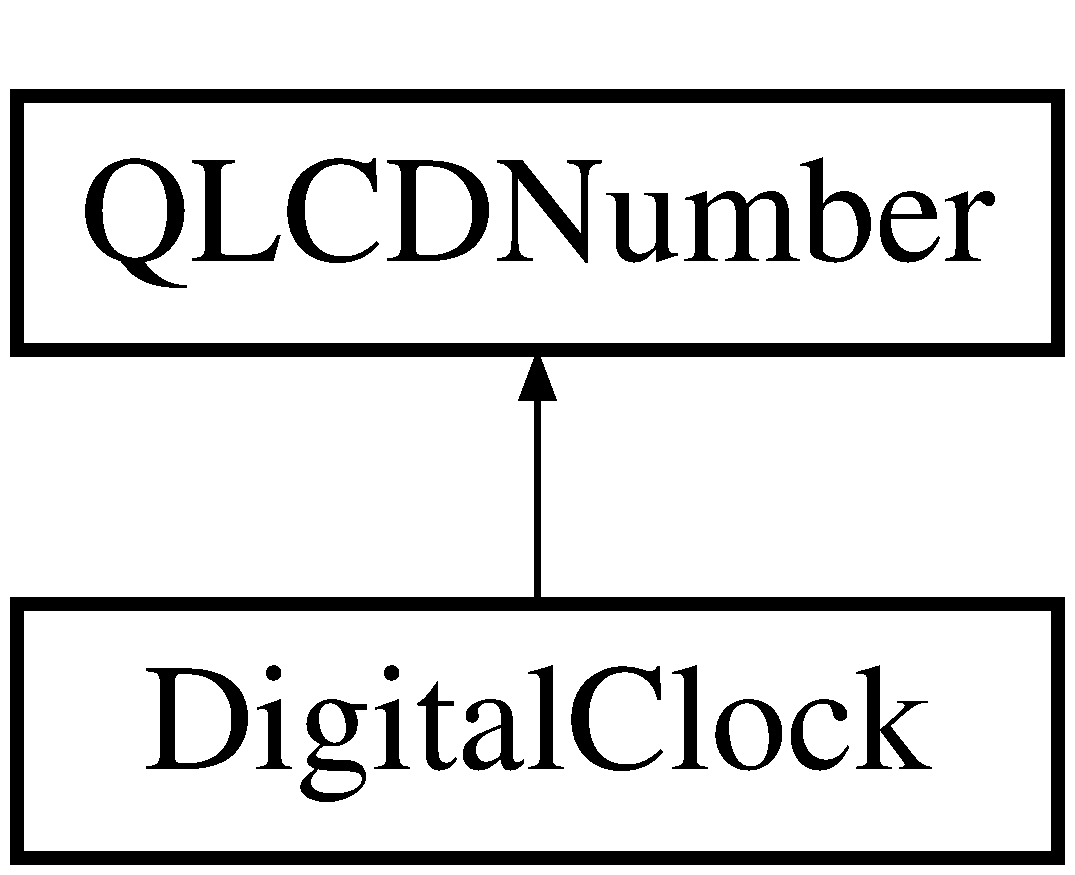
\includegraphics[height=2.000000cm]{class_digital_clock}
\end{center}
\end{figure}
\subsection*{Public Member Functions}
\begin{DoxyCompactItemize}
\item 
\hypertarget{class_digital_clock_a1df69f177d5defdd5029ff2e6b7cb564}{}{\bfseries Digital\+Clock} (Q\+Widget $\ast$parent=0)\label{class_digital_clock_a1df69f177d5defdd5029ff2e6b7cb564}

\item 
\hypertarget{class_digital_clock_a0348581b5afca93efcfd988c63c4a999}{}void {\bfseries start} (int time=0)\label{class_digital_clock_a0348581b5afca93efcfd988c63c4a999}

\item 
\hypertarget{class_digital_clock_ac0122344e8fa3b1fce88571163f6cd10}{}void {\bfseries stop} ()\label{class_digital_clock_ac0122344e8fa3b1fce88571163f6cd10}

\item 
\hypertarget{class_digital_clock_af513f31cd78362b5024753e4087ffde4}{}int {\bfseries get\+Time} ()\label{class_digital_clock_af513f31cd78362b5024753e4087ffde4}

\end{DoxyCompactItemize}


\subsection{Detailed Description}
Projeto\+: Maze Versao\+: 1.\+0b Autores\+: Leno Raimundo 

Definition at line 16 of file digitalclock.\+h.



The documentation for this class was generated from the following files\+:\begin{DoxyCompactItemize}
\item 
digitalclock.\+h\item 
digitalclock.\+cpp\end{DoxyCompactItemize}

\hypertarget{class_game}{}\section{Game Class Reference}
\label{class_game}\index{Game@{Game}}


Gerencia o jogo.  




{\ttfamily \#include $<$game.\+h$>$}

Inheritance diagram for Game\+:\begin{figure}[H]
\begin{center}
\leavevmode
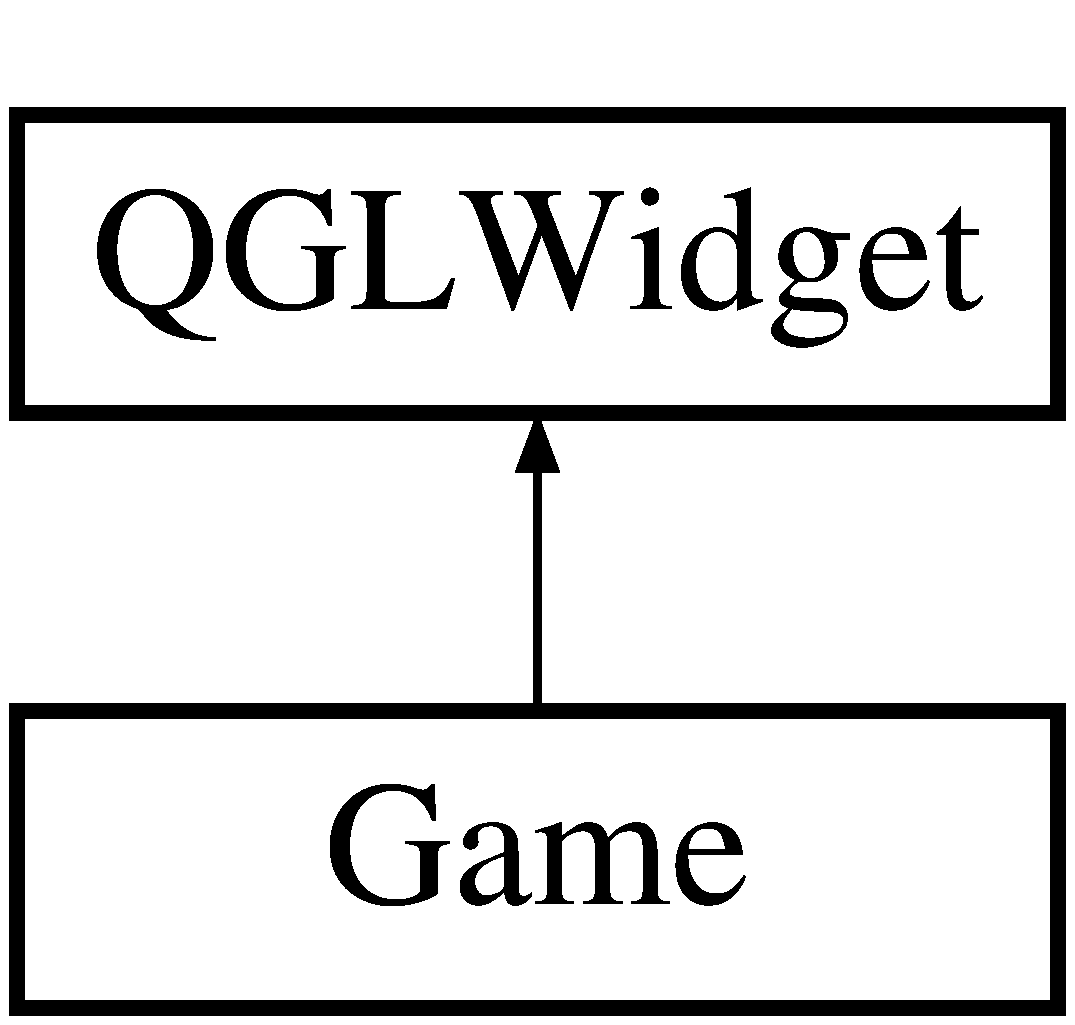
\includegraphics[height=2.000000cm]{class_game}
\end{center}
\end{figure}
\subsection*{Classes}
\begin{DoxyCompactItemize}
\item 
struct \hyperlink{struct_game_1_1_rank}{Rank}
\end{DoxyCompactItemize}
\subsection*{Public Types}
\begin{DoxyCompactItemize}
\item 
\hypertarget{class_game_aa9e701b2208301d5a5a67816ea54fe19}{}enum \hyperlink{class_game_aa9e701b2208301d5a5a67816ea54fe19}{Dificuldade} \{ {\bfseries Facil}, 
{\bfseries Medio}, 
{\bfseries Dificil}
 \}\label{class_game_aa9e701b2208301d5a5a67816ea54fe19}

\begin{DoxyCompactList}\small\item\em Define os niveis de dificuldade do jogo. \end{DoxyCompactList}\item 
\hypertarget{class_game_a78224b33425ca8e37cc762f8a181663e}{}enum \hyperlink{class_game_a78224b33425ca8e37cc762f8a181663e}{Mode} \{ {\bfseries Carreira}, 
{\bfseries Multiplayer}, 
{\bfseries Competir}, 
{\bfseries Treinar}
 \}\label{class_game_a78224b33425ca8e37cc762f8a181663e}

\begin{DoxyCompactList}\small\item\em Define os modos de jogo. \end{DoxyCompactList}\end{DoxyCompactItemize}
\subsection*{Public Member Functions}
\begin{DoxyCompactItemize}
\item 
void \hyperlink{class_game_a290ed80541953c02d4012feae9cf84b4}{set\+Show\+Labirinto} (bool yes=true)
\begin{DoxyCompactList}\small\item\em Exibe ou oculta o labirinto. \end{DoxyCompactList}\item 
void \hyperlink{class_game_a74afd2e4820b0113a1276ba866e5e689}{set\+Wall\+Color} (const \hyperlink{class_color}{Color} \&color)
\begin{DoxyCompactList}\small\item\em Define a cor da parede. \end{DoxyCompactList}\item 
void \hyperlink{class_game_ae2c8fe91e4c6c7e7e49149bc70e7a5c8}{set\+Cell\+Color} (const \hyperlink{class_color}{Color} \&color)
\begin{DoxyCompactList}\small\item\em Define a cor da celula. \end{DoxyCompactList}\item 
void \hyperlink{class_game_a68e69f6f417f07c7f7bfc7e5660d23ab}{set\+Mode} (\hyperlink{class_game_a78224b33425ca8e37cc762f8a181663e}{Mode} mode)
\begin{DoxyCompactList}\small\item\em Define o modo de jogo. \end{DoxyCompactList}\item 
void \hyperlink{class_game_aaa49bf77525ace364d84eb5840fb7f16}{set\+Dificuldade} (\hyperlink{class_game_aa9e701b2208301d5a5a67816ea54fe19}{Dificuldade} dif)
\begin{DoxyCompactList}\small\item\em Define a dificuldade do jogo. \end{DoxyCompactList}\item 
void \hyperlink{class_game_a32ec249abb13c2d4f45f07003046536c}{set\+Wall\+Thickness} (int thickness=1)
\begin{DoxyCompactList}\small\item\em Define a espessura da parede. \end{DoxyCompactList}\item 
void \hyperlink{class_game_a2116158681dfa5fdb17e1ebbadd3348e}{set\+Cell\+Size} (int size=10)
\begin{DoxyCompactList}\small\item\em Define o tamanho de cada celula do labirinto. \end{DoxyCompactList}\item 
\hypertarget{class_game_a3d9b98f7c4a96ecf578f75b96c9f0e90}{}void \hyperlink{class_game_a3d9b98f7c4a96ecf578f75b96c9f0e90}{start} ()\label{class_game_a3d9b98f7c4a96ecf578f75b96c9f0e90}

\begin{DoxyCompactList}\small\item\em Inicia o jogo. \end{DoxyCompactList}\item 
\hypertarget{class_game_a17fbb36fd4a2085f9ff4f1fa93d7d08b}{}void \hyperlink{class_game_a17fbb36fd4a2085f9ff4f1fa93d7d08b}{stop} ()\label{class_game_a17fbb36fd4a2085f9ff4f1fa93d7d08b}

\begin{DoxyCompactList}\small\item\em Para o jogo. \end{DoxyCompactList}\item 
bool \hyperlink{class_game_abb31098c8d016b98888fe9acac497fcb}{is\+Running} () const 
\begin{DoxyCompactList}\small\item\em Checa se o jogo esta em andamento. \end{DoxyCompactList}\item 
void \hyperlink{class_game_ad957f89ebf5557d687332737f5c48174}{set\+Show\+Path} (bool yes)
\begin{DoxyCompactList}\small\item\em Oculta ou exibe o caminho para sair do labirinto. \end{DoxyCompactList}\item 
void \hyperlink{class_game_acf0eab33d0720829856f04df97ae0b60}{set\+Show\+Player1} (bool yes)
\begin{DoxyCompactList}\small\item\em Oculta ou mostra o player1\+\_\+. \end{DoxyCompactList}\item 
void \hyperlink{class_game_a8c3fb62db4b6712d32dc02897464ef77}{set\+Show\+Player2} (bool yes)
\begin{DoxyCompactList}\small\item\em Oculta ou mostra o player2\+\_\+. \end{DoxyCompactList}\item 
bool \hyperlink{class_game_afc0740e2ebbf574081ba72894ffb167d}{get\+Show\+Path} () const 
\begin{DoxyCompactList}\small\item\em Indica se o caminho de saida esta ou nao sendo exibido. \end{DoxyCompactList}\item 
\hyperlink{class_rect}{Rect} \hyperlink{class_game_a5a0887d56454e9f31f800018f211ab1f}{get\+View\+Rect} () const 
\begin{DoxyCompactList}\small\item\em get\+View\+Rect \end{DoxyCompactList}\item 
\hypertarget{class_game_a4d1eb4468fe2a307fa7ca738dd7cfa40}{}void {\bfseries set\+View\+Rect} (const \hyperlink{class_rect}{Rect} \&rect)\label{class_game_a4d1eb4468fe2a307fa7ca738dd7cfa40}

\item 
\hypertarget{class_game_a741d01349d27c8916d6e9975d9c5b470}{}\hyperlink{class_main_window}{Main\+Window} $\ast$ {\bfseries get\+Main\+Window} ()\label{class_game_a741d01349d27c8916d6e9975d9c5b470}

\item 
\hypertarget{class_game_ae9c76f7611a410ac2c92df34cff50a41}{}void {\bfseries set\+Main\+Window} (\hyperlink{class_main_window}{Main\+Window} $\ast$main\+\_\+window)\label{class_game_ae9c76f7611a410ac2c92df34cff50a41}

\item 
void \hyperlink{class_game_a178202f60562a3e55ad721dfb03aff09}{Ler\+\_\+\+Rank} ()
\begin{DoxyCompactList}\small\item\em Ler\+\_\+\+Rank é responsável por fazer a leitura do rank. \end{DoxyCompactList}\item 
\hypertarget{class_game_af8abce48250bf82bc64e30ecc4f2074b}{}std\+::vector$<$ \hyperlink{struct_game_1_1_rank}{Rank} $>$ {\bfseries get\+Rank} () const \label{class_game_af8abce48250bf82bc64e30ecc4f2074b}

\item 
void \hyperlink{class_game_a6b565543a6eaf08a583a9944e8e48d5e}{Ranke} ()
\begin{DoxyCompactList}\small\item\em Ranke é responsável por imprimir no arquivo txt o rank. \end{DoxyCompactList}\end{DoxyCompactItemize}
\subsection*{Static Public Member Functions}
\begin{DoxyCompactItemize}
\item 
static \hyperlink{class_game}{Game} \& \hyperlink{class_game_ab5b377b52d78849aed162538121a20a0}{get\+Instance} ()
\begin{DoxyCompactList}\small\item\em Obtem a referencia desta classe. \end{DoxyCompactList}\end{DoxyCompactItemize}
\subsection*{Protected Slots}
\begin{DoxyCompactItemize}
\item 
\hypertarget{class_game_af79d7cfc146a74d69fe2cbc9f39ddd54}{}void {\bfseries update\+Player1\+Pos} ()\label{class_game_af79d7cfc146a74d69fe2cbc9f39ddd54}

\item 
\hypertarget{class_game_a73139d0f4c34ebfca2b79877d552a39d}{}void {\bfseries update\+Player2\+Pos} ()\label{class_game_a73139d0f4c34ebfca2b79877d552a39d}

\item 
\hypertarget{class_game_ac71e0aadacf88a71f644f4accc1d5d0c}{}void {\bfseries update\+O\+Ground\+Color} ()\label{class_game_ac71e0aadacf88a71f644f4accc1d5d0c}

\end{DoxyCompactItemize}
\subsection*{Protected Member Functions}
\begin{DoxyCompactItemize}
\item 
\hypertarget{class_game_a94d3832f6cd4ea6fe77127b5ce416e08}{}void {\bfseries initialize\+G\+L} ()\label{class_game_a94d3832f6cd4ea6fe77127b5ce416e08}

\item 
\hypertarget{class_game_ae0e64dfe8c1cdc82700cdad1ebcb0488}{}void {\bfseries resize\+G\+L} (int w, int h)\label{class_game_ae0e64dfe8c1cdc82700cdad1ebcb0488}

\item 
\hypertarget{class_game_a893aebaba4c902d2b028cc32a8ed75e9}{}void {\bfseries paint\+G\+L} ()\label{class_game_a893aebaba4c902d2b028cc32a8ed75e9}

\item 
\hypertarget{class_game_a704ba119948eebd1b6dfc547de967796}{}void {\bfseries mouse\+Press\+Event} (Q\+Mouse\+Event $\ast$event)\label{class_game_a704ba119948eebd1b6dfc547de967796}

\item 
\hypertarget{class_game_ad761e49ff42758930e76b477d08ba068}{}void {\bfseries mouse\+Move\+Event} (Q\+Mouse\+Event $\ast$event)\label{class_game_ad761e49ff42758930e76b477d08ba068}

\item 
\hypertarget{class_game_a08d72c91a6daedc8fa48194253f5e567}{}void {\bfseries key\+Press\+Event} (Q\+Key\+Event $\ast$event)\label{class_game_a08d72c91a6daedc8fa48194253f5e567}

\end{DoxyCompactItemize}


\subsection{Detailed Description}
Gerencia o jogo. 

Definition at line 32 of file game.\+h.



\subsection{Member Function Documentation}
\hypertarget{class_game_ab5b377b52d78849aed162538121a20a0}{}\index{Game@{Game}!get\+Instance@{get\+Instance}}
\index{get\+Instance@{get\+Instance}!Game@{Game}}
\subsubsection[{get\+Instance}]{\setlength{\rightskip}{0pt plus 5cm}static {\bf Game}\& Game\+::get\+Instance (
\begin{DoxyParamCaption}
{}
\end{DoxyParamCaption}
)\hspace{0.3cm}{\ttfamily [inline]}, {\ttfamily [static]}}\label{class_game_ab5b377b52d78849aed162538121a20a0}


Obtem a referencia desta classe. 

\begin{DoxyReturn}{Returns}
a referencia desta classe 
\end{DoxyReturn}


Definition at line 67 of file game.\+h.

\hypertarget{class_game_afc0740e2ebbf574081ba72894ffb167d}{}\index{Game@{Game}!get\+Show\+Path@{get\+Show\+Path}}
\index{get\+Show\+Path@{get\+Show\+Path}!Game@{Game}}
\subsubsection[{get\+Show\+Path}]{\setlength{\rightskip}{0pt plus 5cm}bool Game\+::get\+Show\+Path (
\begin{DoxyParamCaption}
{}
\end{DoxyParamCaption}
) const\hspace{0.3cm}{\ttfamily [inline]}}\label{class_game_afc0740e2ebbf574081ba72894ffb167d}


Indica se o caminho de saida esta ou nao sendo exibido. 

\begin{DoxyReturn}{Returns}
true se o caminho de saida esta sendo exibido, senao retorna false 
\end{DoxyReturn}


Definition at line 159 of file game.\+h.

\hypertarget{class_game_a5a0887d56454e9f31f800018f211ab1f}{}\index{Game@{Game}!get\+View\+Rect@{get\+View\+Rect}}
\index{get\+View\+Rect@{get\+View\+Rect}!Game@{Game}}
\subsubsection[{get\+View\+Rect}]{\setlength{\rightskip}{0pt plus 5cm}{\bf Rect} Game\+::get\+View\+Rect (
\begin{DoxyParamCaption}
{}
\end{DoxyParamCaption}
) const\hspace{0.3cm}{\ttfamily [inline]}}\label{class_game_a5a0887d56454e9f31f800018f211ab1f}


get\+View\+Rect 

\begin{DoxyReturn}{Returns}

\end{DoxyReturn}


Definition at line 165 of file game.\+h.

\hypertarget{class_game_abb31098c8d016b98888fe9acac497fcb}{}\index{Game@{Game}!is\+Running@{is\+Running}}
\index{is\+Running@{is\+Running}!Game@{Game}}
\subsubsection[{is\+Running}]{\setlength{\rightskip}{0pt plus 5cm}bool Game\+::is\+Running (
\begin{DoxyParamCaption}
{}
\end{DoxyParamCaption}
) const\hspace{0.3cm}{\ttfamily [inline]}}\label{class_game_abb31098c8d016b98888fe9acac497fcb}


Checa se o jogo esta em andamento. 

\begin{DoxyReturn}{Returns}
true se o jogo esta em andamento, senao retorna false 
\end{DoxyReturn}


Definition at line 135 of file game.\+h.

\hypertarget{class_game_a178202f60562a3e55ad721dfb03aff09}{}\index{Game@{Game}!Ler\+\_\+\+Rank@{Ler\+\_\+\+Rank}}
\index{Ler\+\_\+\+Rank@{Ler\+\_\+\+Rank}!Game@{Game}}
\subsubsection[{Ler\+\_\+\+Rank}]{\setlength{\rightskip}{0pt plus 5cm}void Game\+::\+Ler\+\_\+\+Rank (
\begin{DoxyParamCaption}
{}
\end{DoxyParamCaption}
)}\label{class_game_a178202f60562a3e55ad721dfb03aff09}


Ler\+\_\+\+Rank é responsável por fazer a leitura do rank. 

\begin{DoxyReturn}{Returns}

\end{DoxyReturn}


Definition at line 949 of file game.\+cpp.

\hypertarget{class_game_a6b565543a6eaf08a583a9944e8e48d5e}{}\index{Game@{Game}!Ranke@{Ranke}}
\index{Ranke@{Ranke}!Game@{Game}}
\subsubsection[{Ranke}]{\setlength{\rightskip}{0pt plus 5cm}void Game\+::\+Ranke (
\begin{DoxyParamCaption}
{}
\end{DoxyParamCaption}
)}\label{class_game_a6b565543a6eaf08a583a9944e8e48d5e}


Ranke é responsável por imprimir no arquivo txt o rank. 

\begin{DoxyReturn}{Returns}

\end{DoxyReturn}


Definition at line 987 of file game.\+cpp.

\hypertarget{class_game_ae2c8fe91e4c6c7e7e49149bc70e7a5c8}{}\index{Game@{Game}!set\+Cell\+Color@{set\+Cell\+Color}}
\index{set\+Cell\+Color@{set\+Cell\+Color}!Game@{Game}}
\subsubsection[{set\+Cell\+Color}]{\setlength{\rightskip}{0pt plus 5cm}void Game\+::set\+Cell\+Color (
\begin{DoxyParamCaption}
\item[{const {\bf Color} \&}]{color}
\end{DoxyParamCaption}
)\hspace{0.3cm}{\ttfamily [inline]}}\label{class_game_ae2c8fe91e4c6c7e7e49149bc70e7a5c8}


Define a cor da celula. 


\begin{DoxyParams}{Parameters}
{\em color} & uma cor qualquer \\
\hline
\end{DoxyParams}


Definition at line 95 of file game.\+h.

\hypertarget{class_game_a2116158681dfa5fdb17e1ebbadd3348e}{}\index{Game@{Game}!set\+Cell\+Size@{set\+Cell\+Size}}
\index{set\+Cell\+Size@{set\+Cell\+Size}!Game@{Game}}
\subsubsection[{set\+Cell\+Size}]{\setlength{\rightskip}{0pt plus 5cm}void Game\+::set\+Cell\+Size (
\begin{DoxyParamCaption}
\item[{int}]{size = {\ttfamily 10}}
\end{DoxyParamCaption}
)\hspace{0.3cm}{\ttfamily [inline]}}\label{class_game_a2116158681dfa5fdb17e1ebbadd3348e}


Define o tamanho de cada celula do labirinto. 


\begin{DoxyParams}{Parameters}
{\em size} & o tamanho da celula \\
\hline
\end{DoxyParams}


Definition at line 119 of file game.\+h.

\hypertarget{class_game_aaa49bf77525ace364d84eb5840fb7f16}{}\index{Game@{Game}!set\+Dificuldade@{set\+Dificuldade}}
\index{set\+Dificuldade@{set\+Dificuldade}!Game@{Game}}
\subsubsection[{set\+Dificuldade}]{\setlength{\rightskip}{0pt plus 5cm}void Game\+::set\+Dificuldade (
\begin{DoxyParamCaption}
\item[{{\bf Game\+::\+Dificuldade}}]{dif}
\end{DoxyParamCaption}
)}\label{class_game_aaa49bf77525ace364d84eb5840fb7f16}


Define a dificuldade do jogo. 


\begin{DoxyParams}{Parameters}
{\em dif} & uma dificuldade do jogo \\
\hline
\end{DoxyParams}


Definition at line 74 of file game.\+cpp.

\hypertarget{class_game_a68e69f6f417f07c7f7bfc7e5660d23ab}{}\index{Game@{Game}!set\+Mode@{set\+Mode}}
\index{set\+Mode@{set\+Mode}!Game@{Game}}
\subsubsection[{set\+Mode}]{\setlength{\rightskip}{0pt plus 5cm}void Game\+::set\+Mode (
\begin{DoxyParamCaption}
\item[{{\bf Game\+::\+Mode}}]{mode}
\end{DoxyParamCaption}
)}\label{class_game_a68e69f6f417f07c7f7bfc7e5660d23ab}


Define o modo de jogo. 


\begin{DoxyParams}{Parameters}
{\em mode} & um modo de jogo \\
\hline
\end{DoxyParams}


Definition at line 66 of file game.\+cpp.

\hypertarget{class_game_a290ed80541953c02d4012feae9cf84b4}{}\index{Game@{Game}!set\+Show\+Labirinto@{set\+Show\+Labirinto}}
\index{set\+Show\+Labirinto@{set\+Show\+Labirinto}!Game@{Game}}
\subsubsection[{set\+Show\+Labirinto}]{\setlength{\rightskip}{0pt plus 5cm}void Game\+::set\+Show\+Labirinto (
\begin{DoxyParamCaption}
\item[{bool}]{yes = {\ttfamily true}}
\end{DoxyParamCaption}
)\hspace{0.3cm}{\ttfamily [inline]}}\label{class_game_a290ed80541953c02d4012feae9cf84b4}


Exibe ou oculta o labirinto. 


\begin{DoxyParams}{Parameters}
{\em yes} & Se true, exibe o labirinto, senao nao exibe. \\
\hline
\end{DoxyParams}


Definition at line 83 of file game.\+h.

\hypertarget{class_game_ad957f89ebf5557d687332737f5c48174}{}\index{Game@{Game}!set\+Show\+Path@{set\+Show\+Path}}
\index{set\+Show\+Path@{set\+Show\+Path}!Game@{Game}}
\subsubsection[{set\+Show\+Path}]{\setlength{\rightskip}{0pt plus 5cm}void Game\+::set\+Show\+Path (
\begin{DoxyParamCaption}
\item[{bool}]{yes}
\end{DoxyParamCaption}
)\hspace{0.3cm}{\ttfamily [inline]}}\label{class_game_ad957f89ebf5557d687332737f5c48174}


Oculta ou exibe o caminho para sair do labirinto. 


\begin{DoxyParams}{Parameters}
{\em yes} & se true, revela o caminho, senao nao revela. \\
\hline
\end{DoxyParams}


Definition at line 140 of file game.\+h.

\hypertarget{class_game_acf0eab33d0720829856f04df97ae0b60}{}\index{Game@{Game}!set\+Show\+Player1@{set\+Show\+Player1}}
\index{set\+Show\+Player1@{set\+Show\+Player1}!Game@{Game}}
\subsubsection[{set\+Show\+Player1}]{\setlength{\rightskip}{0pt plus 5cm}void Game\+::set\+Show\+Player1 (
\begin{DoxyParamCaption}
\item[{bool}]{yes}
\end{DoxyParamCaption}
)\hspace{0.3cm}{\ttfamily [inline]}}\label{class_game_acf0eab33d0720829856f04df97ae0b60}


Oculta ou mostra o player1\+\_\+. 


\begin{DoxyParams}{Parameters}
{\em yes} & se true, mostra o player1, senao nao mostra \\
\hline
\end{DoxyParams}


Definition at line 146 of file game.\+h.

\hypertarget{class_game_a8c3fb62db4b6712d32dc02897464ef77}{}\index{Game@{Game}!set\+Show\+Player2@{set\+Show\+Player2}}
\index{set\+Show\+Player2@{set\+Show\+Player2}!Game@{Game}}
\subsubsection[{set\+Show\+Player2}]{\setlength{\rightskip}{0pt plus 5cm}void Game\+::set\+Show\+Player2 (
\begin{DoxyParamCaption}
\item[{bool}]{yes}
\end{DoxyParamCaption}
)\hspace{0.3cm}{\ttfamily [inline]}}\label{class_game_a8c3fb62db4b6712d32dc02897464ef77}


Oculta ou mostra o player2\+\_\+. 


\begin{DoxyParams}{Parameters}
{\em yes} & se true, mostra o player2, senao nao mostra \\
\hline
\end{DoxyParams}


Definition at line 152 of file game.\+h.

\hypertarget{class_game_a74afd2e4820b0113a1276ba866e5e689}{}\index{Game@{Game}!set\+Wall\+Color@{set\+Wall\+Color}}
\index{set\+Wall\+Color@{set\+Wall\+Color}!Game@{Game}}
\subsubsection[{set\+Wall\+Color}]{\setlength{\rightskip}{0pt plus 5cm}void Game\+::set\+Wall\+Color (
\begin{DoxyParamCaption}
\item[{const {\bf Color} \&}]{color}
\end{DoxyParamCaption}
)\hspace{0.3cm}{\ttfamily [inline]}}\label{class_game_a74afd2e4820b0113a1276ba866e5e689}


Define a cor da parede. 


\begin{DoxyParams}{Parameters}
{\em color} & uma cor qualquer \\
\hline
\end{DoxyParams}


Definition at line 89 of file game.\+h.

\hypertarget{class_game_a32ec249abb13c2d4f45f07003046536c}{}\index{Game@{Game}!set\+Wall\+Thickness@{set\+Wall\+Thickness}}
\index{set\+Wall\+Thickness@{set\+Wall\+Thickness}!Game@{Game}}
\subsubsection[{set\+Wall\+Thickness}]{\setlength{\rightskip}{0pt plus 5cm}void Game\+::set\+Wall\+Thickness (
\begin{DoxyParamCaption}
\item[{int}]{thickness = {\ttfamily 1}}
\end{DoxyParamCaption}
)\hspace{0.3cm}{\ttfamily [inline]}}\label{class_game_a32ec249abb13c2d4f45f07003046536c}


Define a espessura da parede. 


\begin{DoxyParams}{Parameters}
{\em thickness} & a espessura da parede. \\
\hline
\end{DoxyParams}


Definition at line 113 of file game.\+h.



The documentation for this class was generated from the following files\+:\begin{DoxyCompactItemize}
\item 
game.\+h\item 
game.\+cpp\end{DoxyCompactItemize}

\hypertarget{class_labirinto}{}\section{Labirinto Class Reference}
\label{class_labirinto}\index{Labirinto@{Labirinto}}


Classe para criar um labirinto.  




{\ttfamily \#include $<$labirinto.\+h$>$}

\subsection*{Classes}
\begin{DoxyCompactItemize}
\item 
struct \hyperlink{struct_labirinto_1_1_cell}{Cell}
\begin{DoxyCompactList}\small\item\em Uma celula do labirinto. Uma celula representa uma posicao unica dentro de um labirinto. Cada celula pode ter ate 4 paredes erguidas, e pelo menos duas paredes dela sao compartilhadas com outras celulas. \end{DoxyCompactList}\end{DoxyCompactItemize}
\subsection*{Public Types}
\begin{DoxyCompactItemize}
\item 
enum \hyperlink{class_labirinto_ab6ffda1571ea6394c382e12b4bb4c336}{Wall} \{ \\*
{\bfseries None} = 0, 
\hyperlink{class_labirinto_ab6ffda1571ea6394c382e12b4bb4c336a51cd26ae8c945f233f769e8f825576b7}{North\+Wall} = 1, 
\hyperlink{class_labirinto_ab6ffda1571ea6394c382e12b4bb4c336aa4d6ec05499a34df7626c5163cb8c6c6}{East\+Wall} = 2, 
\hyperlink{class_labirinto_ab6ffda1571ea6394c382e12b4bb4c336a0b35a31c56ee4c65e64e479bd6b77d43}{South\+Wall} = 4, 
\\*
\hyperlink{class_labirinto_ab6ffda1571ea6394c382e12b4bb4c336a5f71f0a5c304ca89e2aee5d8159b6d39}{West\+Wall} = 8
 \}
\begin{DoxyCompactList}\small\item\em As 4 possiveis paredes de uma celula. \end{DoxyCompactList}\end{DoxyCompactItemize}
\subsection*{Public Member Functions}
\begin{DoxyCompactItemize}
\item 
\hyperlink{class_labirinto_a086420b862b2009f7da95967a075bd36}{Labirinto} (int \hyperlink{class_labirinto_a4f8c7a42d8a5edad12482f4d2110626c}{rows}, int \hyperlink{class_labirinto_a6614a825d5e93ec1c053003a804ce2a7}{columns})
\begin{DoxyCompactList}\small\item\em Cria um labirinto. \end{DoxyCompactList}\item 
bool \hyperlink{class_labirinto_a02a05067a6380b1e720da444bb4718f7}{build} ()
\begin{DoxyCompactList}\small\item\em Constroi o labirinto. O processo de construcao consiste em criar uma entrada e saida, o caminho de saida e suas ramificacoes de modo a tornar o labirinto totalmente conexo. \end{DoxyCompactList}\item 
std\+::vector$<$ \hyperlink{struct_labirinto_1_1_cell}{Cell} $>$ \hyperlink{class_labirinto_a5560f3c1a18c95009ced3e855d53bebb}{get\+Path} (const \hyperlink{struct_labirinto_1_1_cell}{Cell} \&c1, const \hyperlink{struct_labirinto_1_1_cell}{Cell} \&c2) const 
\begin{DoxyCompactList}\small\item\em Obtem o caminho para sair do labirinto. \end{DoxyCompactList}\item 
int \hyperlink{class_labirinto_a9b6d4d4b8a3b53aa10761c8fc0e325d9}{get\+Destroyed\+Walls} (const \hyperlink{struct_labirinto_1_1_cell}{Cell} \&cell) const 
\begin{DoxyCompactList}\small\item\em Obtem as paredes derrubadas de uma celula. Para extrair as paredes do inteiro retornado, use o operador binario \&. Por exemplo, supondo que a funcao retorne 3, para saber se a parede Norte esta destruida, use a expressao \textquotesingle{}3 \& \hyperlink{class_labirinto_ab6ffda1571ea6394c382e12b4bb4c336a51cd26ae8c945f233f769e8f825576b7}{Labirinto\+::\+North\+Wall}\textquotesingle{}. \end{DoxyCompactList}\item 
bool \hyperlink{class_labirinto_a8054ff4d8c0712dffad07768bdcb1b6d}{is\+Cell\+Valid} (const \hyperlink{struct_labirinto_1_1_cell}{Cell} \&cell) const 
\begin{DoxyCompactList}\small\item\em Verifica se uma celula e valida, ou seja, esta no labirinto. \end{DoxyCompactList}\item 
std\+::vector$<$ \hyperlink{struct_labirinto_1_1_cell}{Cell} $>$ \hyperlink{class_labirinto_a49eb1b0dd3bdb40ff020dfff1f5741be}{get\+Neighbors} (const \hyperlink{struct_labirinto_1_1_cell}{Cell} \&cell, int walls) const 
\begin{DoxyCompactList}\small\item\em Obtem as celulas vizinhas em relacao as paredes especificadas. \end{DoxyCompactList}\item 
bool \hyperlink{class_labirinto_affebfa176e56784b0ca6e1c8f5a9d1dc}{is\+Wall\+Shared} (\hyperlink{class_labirinto_ab6ffda1571ea6394c382e12b4bb4c336}{Wall} wall, const \hyperlink{struct_labirinto_1_1_cell}{Cell} \&cell, \hyperlink{struct_labirinto_1_1_cell}{Cell} $\ast$other\+\_\+cell=N\+U\+L\+L) const 
\begin{DoxyCompactList}\small\item\em Verifica se uma parede e compartilhada, ou seja, pertence a duas celulas. Se a parede for compartilhada e o parametro opcional nao for nulo, entao ele recebe a outra celula que possui a parede. Note que uma parede nao e compartilhada se, e somente se, ela delimita o labirinto. \end{DoxyCompactList}\item 
int \hyperlink{class_labirinto_a4f8c7a42d8a5edad12482f4d2110626c}{rows} () const 
\begin{DoxyCompactList}\small\item\em Obtem o numero de linhas do labirinto. \end{DoxyCompactList}\item 
int \hyperlink{class_labirinto_a6614a825d5e93ec1c053003a804ce2a7}{columns} () const 
\begin{DoxyCompactList}\small\item\em Obtem o numero de colunas do labirinto. \end{DoxyCompactList}\end{DoxyCompactItemize}
\subsection*{Static Public Member Functions}
\begin{DoxyCompactItemize}
\item 
static \hyperlink{class_labirinto_ab6ffda1571ea6394c382e12b4bb4c336}{Wall} \hyperlink{class_labirinto_a567e53ede46c4341dce6e44c2e7637e4}{get\+Opposite\+Wall} (\hyperlink{class_labirinto_ab6ffda1571ea6394c382e12b4bb4c336}{Wall} wall)
\begin{DoxyCompactList}\small\item\em Obtem a parede oposta a uma parede. Por exemplo, a parede oposta a parede Norte e a parede Sul, e a parede oposta a parede Leste e a parede Oeste. \end{DoxyCompactList}\item 
static \hyperlink{class_labirinto_ab6ffda1571ea6394c382e12b4bb4c336}{Wall} \hyperlink{class_labirinto_ac75602d107390976f691cb0865f81ec5}{pick\+Wall\+Randomly} (int walls)
\begin{DoxyCompactList}\small\item\em Escolhe aleatoriamente uma parede. \end{DoxyCompactList}\end{DoxyCompactItemize}


\subsection{Detailed Description}
Classe para criar um labirinto. 

Projeto\+: Maze Versao\+: 1.\+0b Autores\+: Leno Raimundo 

Definition at line 17 of file labirinto.\+h.



\subsection{Member Enumeration Documentation}
\hypertarget{class_labirinto_ab6ffda1571ea6394c382e12b4bb4c336}{}\index{Labirinto@{Labirinto}!Wall@{Wall}}
\index{Wall@{Wall}!Labirinto@{Labirinto}}
\subsubsection[{Wall}]{\setlength{\rightskip}{0pt plus 5cm}enum {\bf Labirinto\+::\+Wall}}\label{class_labirinto_ab6ffda1571ea6394c382e12b4bb4c336}


As 4 possiveis paredes de uma celula. 

\begin{Desc}
\item[Enumerator]\par
\begin{description}
\index{North\+Wall@{North\+Wall}!Labirinto@{Labirinto}}\index{Labirinto@{Labirinto}!North\+Wall@{North\+Wall}}\item[{\em 
\hypertarget{class_labirinto_ab6ffda1571ea6394c382e12b4bb4c336a51cd26ae8c945f233f769e8f825576b7}{}North\+Wall\label{class_labirinto_ab6ffda1571ea6394c382e12b4bb4c336a51cd26ae8c945f233f769e8f825576b7}
}]Parede Norte. \index{East\+Wall@{East\+Wall}!Labirinto@{Labirinto}}\index{Labirinto@{Labirinto}!East\+Wall@{East\+Wall}}\item[{\em 
\hypertarget{class_labirinto_ab6ffda1571ea6394c382e12b4bb4c336aa4d6ec05499a34df7626c5163cb8c6c6}{}East\+Wall\label{class_labirinto_ab6ffda1571ea6394c382e12b4bb4c336aa4d6ec05499a34df7626c5163cb8c6c6}
}]Parede Leste. \index{South\+Wall@{South\+Wall}!Labirinto@{Labirinto}}\index{Labirinto@{Labirinto}!South\+Wall@{South\+Wall}}\item[{\em 
\hypertarget{class_labirinto_ab6ffda1571ea6394c382e12b4bb4c336a0b35a31c56ee4c65e64e479bd6b77d43}{}South\+Wall\label{class_labirinto_ab6ffda1571ea6394c382e12b4bb4c336a0b35a31c56ee4c65e64e479bd6b77d43}
}]Parede Sul. \index{West\+Wall@{West\+Wall}!Labirinto@{Labirinto}}\index{Labirinto@{Labirinto}!West\+Wall@{West\+Wall}}\item[{\em 
\hypertarget{class_labirinto_ab6ffda1571ea6394c382e12b4bb4c336a5f71f0a5c304ca89e2aee5d8159b6d39}{}West\+Wall\label{class_labirinto_ab6ffda1571ea6394c382e12b4bb4c336a5f71f0a5c304ca89e2aee5d8159b6d39}
}]Parede Oeste. \end{description}
\end{Desc}


Definition at line 23 of file labirinto.\+h.



\subsection{Constructor \& Destructor Documentation}
\hypertarget{class_labirinto_a086420b862b2009f7da95967a075bd36}{}\index{Labirinto@{Labirinto}!Labirinto@{Labirinto}}
\index{Labirinto@{Labirinto}!Labirinto@{Labirinto}}
\subsubsection[{Labirinto}]{\setlength{\rightskip}{0pt plus 5cm}Labirinto\+::\+Labirinto (
\begin{DoxyParamCaption}
\item[{int}]{rows, }
\item[{int}]{columns}
\end{DoxyParamCaption}
)}\label{class_labirinto_a086420b862b2009f7da95967a075bd36}


Cria um labirinto. 


\begin{DoxyParams}{Parameters}
{\em rows} & O numero de linhas, ou seja, o numero de celulas dispostas horizontalmente no labirinto. \\
\hline
{\em columns} & O numero de colunas, ou seja, o numero de celulas dispostas verticalmente no labirinto. \\
\hline
\end{DoxyParams}


Definition at line 14 of file labirinto.\+cpp.



\subsection{Member Function Documentation}
\hypertarget{class_labirinto_a02a05067a6380b1e720da444bb4718f7}{}\index{Labirinto@{Labirinto}!build@{build}}
\index{build@{build}!Labirinto@{Labirinto}}
\subsubsection[{build}]{\setlength{\rightskip}{0pt plus 5cm}bool Labirinto\+::build (
\begin{DoxyParamCaption}
{}
\end{DoxyParamCaption}
)}\label{class_labirinto_a02a05067a6380b1e720da444bb4718f7}


Constroi o labirinto. O processo de construcao consiste em criar uma entrada e saida, o caminho de saida e suas ramificacoes de modo a tornar o labirinto totalmente conexo. 

\begin{DoxyReturn}{Returns}
sempre true. 
\end{DoxyReturn}


Definition at line 36 of file labirinto.\+cpp.

\hypertarget{class_labirinto_a6614a825d5e93ec1c053003a804ce2a7}{}\index{Labirinto@{Labirinto}!columns@{columns}}
\index{columns@{columns}!Labirinto@{Labirinto}}
\subsubsection[{columns}]{\setlength{\rightskip}{0pt plus 5cm}int Labirinto\+::columns (
\begin{DoxyParamCaption}
{}
\end{DoxyParamCaption}
) const\hspace{0.3cm}{\ttfamily [inline]}}\label{class_labirinto_a6614a825d5e93ec1c053003a804ce2a7}


Obtem o numero de colunas do labirinto. 

\begin{DoxyReturn}{Returns}
o numero de colunas do labirinto 
\end{DoxyReturn}


Definition at line 148 of file labirinto.\+h.

\hypertarget{class_labirinto_a9b6d4d4b8a3b53aa10761c8fc0e325d9}{}\index{Labirinto@{Labirinto}!get\+Destroyed\+Walls@{get\+Destroyed\+Walls}}
\index{get\+Destroyed\+Walls@{get\+Destroyed\+Walls}!Labirinto@{Labirinto}}
\subsubsection[{get\+Destroyed\+Walls}]{\setlength{\rightskip}{0pt plus 5cm}int Labirinto\+::get\+Destroyed\+Walls (
\begin{DoxyParamCaption}
\item[{const {\bf Cell} \&}]{cell}
\end{DoxyParamCaption}
) const}\label{class_labirinto_a9b6d4d4b8a3b53aa10761c8fc0e325d9}


Obtem as paredes derrubadas de uma celula. Para extrair as paredes do inteiro retornado, use o operador binario \&. Por exemplo, supondo que a funcao retorne 3, para saber se a parede Norte esta destruida, use a expressao \textquotesingle{}3 \& \hyperlink{class_labirinto_ab6ffda1571ea6394c382e12b4bb4c336a51cd26ae8c945f233f769e8f825576b7}{Labirinto\+::\+North\+Wall}\textquotesingle{}. 


\begin{DoxyParams}{Parameters}
{\em cell} & uma celula do labirinto. \\
\hline
\end{DoxyParams}
\begin{DoxyReturn}{Returns}
um inteiro contendo as paredes destruidas da celula. 
\end{DoxyReturn}


Definition at line 121 of file labirinto.\+cpp.

\hypertarget{class_labirinto_a49eb1b0dd3bdb40ff020dfff1f5741be}{}\index{Labirinto@{Labirinto}!get\+Neighbors@{get\+Neighbors}}
\index{get\+Neighbors@{get\+Neighbors}!Labirinto@{Labirinto}}
\subsubsection[{get\+Neighbors}]{\setlength{\rightskip}{0pt plus 5cm}std\+::vector$<$ {\bf Labirinto\+::\+Cell} $>$ Labirinto\+::get\+Neighbors (
\begin{DoxyParamCaption}
\item[{const {\bf Cell} \&}]{cell, }
\item[{int}]{walls}
\end{DoxyParamCaption}
) const}\label{class_labirinto_a49eb1b0dd3bdb40ff020dfff1f5741be}


Obtem as celulas vizinhas em relacao as paredes especificadas. 


\begin{DoxyParams}{Parameters}
{\em cell} & uma celula do labirinto \\
\hline
{\em walls} & uma ou mais paredes da celula \\
\hline
\end{DoxyParams}
\begin{DoxyReturn}{Returns}
uma lista das celulas vizinhas 
\end{DoxyReturn}


Definition at line 136 of file labirinto.\+cpp.

\hypertarget{class_labirinto_a567e53ede46c4341dce6e44c2e7637e4}{}\index{Labirinto@{Labirinto}!get\+Opposite\+Wall@{get\+Opposite\+Wall}}
\index{get\+Opposite\+Wall@{get\+Opposite\+Wall}!Labirinto@{Labirinto}}
\subsubsection[{get\+Opposite\+Wall}]{\setlength{\rightskip}{0pt plus 5cm}{\bf Labirinto\+::\+Wall} Labirinto\+::get\+Opposite\+Wall (
\begin{DoxyParamCaption}
\item[{{\bf Labirinto\+::\+Wall}}]{wall}
\end{DoxyParamCaption}
)\hspace{0.3cm}{\ttfamily [static]}}\label{class_labirinto_a567e53ede46c4341dce6e44c2e7637e4}


Obtem a parede oposta a uma parede. Por exemplo, a parede oposta a parede Norte e a parede Sul, e a parede oposta a parede Leste e a parede Oeste. 


\begin{DoxyParams}{Parameters}
{\em wall} & uma parede qualquer. \\
\hline
\end{DoxyParams}
\begin{DoxyReturn}{Returns}
a parede oposta a parede especificada. 
\end{DoxyReturn}


Definition at line 213 of file labirinto.\+cpp.

\hypertarget{class_labirinto_a5560f3c1a18c95009ced3e855d53bebb}{}\index{Labirinto@{Labirinto}!get\+Path@{get\+Path}}
\index{get\+Path@{get\+Path}!Labirinto@{Labirinto}}
\subsubsection[{get\+Path}]{\setlength{\rightskip}{0pt plus 5cm}std\+::vector$<$ {\bf Labirinto\+::\+Cell} $>$ Labirinto\+::get\+Path (
\begin{DoxyParamCaption}
\item[{const {\bf Cell} \&}]{c1, }
\item[{const {\bf Cell} \&}]{c2}
\end{DoxyParamCaption}
) const}\label{class_labirinto_a5560f3c1a18c95009ced3e855d53bebb}


Obtem o caminho para sair do labirinto. 


\begin{DoxyParams}{Parameters}
{\em cell} & A celula onde o caminho sera iniciado. \\
\hline
\end{DoxyParams}
\begin{DoxyReturn}{Returns}
Um vetor de celulas que representa o caminho para sair do labirinto. 
\end{DoxyReturn}


Definition at line 79 of file labirinto.\+cpp.

\hypertarget{class_labirinto_a8054ff4d8c0712dffad07768bdcb1b6d}{}\index{Labirinto@{Labirinto}!is\+Cell\+Valid@{is\+Cell\+Valid}}
\index{is\+Cell\+Valid@{is\+Cell\+Valid}!Labirinto@{Labirinto}}
\subsubsection[{is\+Cell\+Valid}]{\setlength{\rightskip}{0pt plus 5cm}bool Labirinto\+::is\+Cell\+Valid (
\begin{DoxyParamCaption}
\item[{const {\bf Cell} \&}]{cell}
\end{DoxyParamCaption}
) const}\label{class_labirinto_a8054ff4d8c0712dffad07768bdcb1b6d}


Verifica se uma celula e valida, ou seja, esta no labirinto. 


\begin{DoxyParams}{Parameters}
{\em cell} & uma celula qualquer. \\
\hline
\end{DoxyParams}
\begin{DoxyReturn}{Returns}
true se a celula especificada e valida, senao retorna false. 
\end{DoxyReturn}


Definition at line 128 of file labirinto.\+cpp.

\hypertarget{class_labirinto_affebfa176e56784b0ca6e1c8f5a9d1dc}{}\index{Labirinto@{Labirinto}!is\+Wall\+Shared@{is\+Wall\+Shared}}
\index{is\+Wall\+Shared@{is\+Wall\+Shared}!Labirinto@{Labirinto}}
\subsubsection[{is\+Wall\+Shared}]{\setlength{\rightskip}{0pt plus 5cm}bool Labirinto\+::is\+Wall\+Shared (
\begin{DoxyParamCaption}
\item[{{\bf Labirinto\+::\+Wall}}]{wall, }
\item[{const {\bf Cell} \&}]{cell, }
\item[{{\bf Labirinto\+::\+Cell} $\ast$}]{other\+\_\+cell = {\ttfamily NULL}}
\end{DoxyParamCaption}
) const}\label{class_labirinto_affebfa176e56784b0ca6e1c8f5a9d1dc}


Verifica se uma parede e compartilhada, ou seja, pertence a duas celulas. Se a parede for compartilhada e o parametro opcional nao for nulo, entao ele recebe a outra celula que possui a parede. Note que uma parede nao e compartilhada se, e somente se, ela delimita o labirinto. 


\begin{DoxyParams}{Parameters}
{\em wall} & uma das paredes da celula especificada \\
\hline
{\em cell} & uma celula do labirinto \\
\hline
{\em other\+\_\+cell} & opcional. Ponteiro que recebera a outra celula que compartilha a parede especificada. \\
\hline
\end{DoxyParams}
\begin{DoxyReturn}{Returns}
true se a parede e compartilhada, senao retorna false. 
\end{DoxyReturn}


Definition at line 159 of file labirinto.\+cpp.

\hypertarget{class_labirinto_ac75602d107390976f691cb0865f81ec5}{}\index{Labirinto@{Labirinto}!pick\+Wall\+Randomly@{pick\+Wall\+Randomly}}
\index{pick\+Wall\+Randomly@{pick\+Wall\+Randomly}!Labirinto@{Labirinto}}
\subsubsection[{pick\+Wall\+Randomly}]{\setlength{\rightskip}{0pt plus 5cm}{\bf Labirinto\+::\+Wall} Labirinto\+::pick\+Wall\+Randomly (
\begin{DoxyParamCaption}
\item[{int}]{walls}
\end{DoxyParamCaption}
)\hspace{0.3cm}{\ttfamily [static]}}\label{class_labirinto_ac75602d107390976f691cb0865f81ec5}


Escolhe aleatoriamente uma parede. 


\begin{DoxyParams}{Parameters}
{\em walls} & as paredes que podem ser escolhidas \\
\hline
\end{DoxyParams}
\begin{DoxyReturn}{Returns}
uma parede 
\end{DoxyReturn}


Definition at line 251 of file labirinto.\+cpp.

\hypertarget{class_labirinto_a4f8c7a42d8a5edad12482f4d2110626c}{}\index{Labirinto@{Labirinto}!rows@{rows}}
\index{rows@{rows}!Labirinto@{Labirinto}}
\subsubsection[{rows}]{\setlength{\rightskip}{0pt plus 5cm}int Labirinto\+::rows (
\begin{DoxyParamCaption}
{}
\end{DoxyParamCaption}
) const\hspace{0.3cm}{\ttfamily [inline]}}\label{class_labirinto_a4f8c7a42d8a5edad12482f4d2110626c}


Obtem o numero de linhas do labirinto. 

\begin{DoxyReturn}{Returns}
o numero de linhas do labirinto 
\end{DoxyReturn}


Definition at line 141 of file labirinto.\+h.



The documentation for this class was generated from the following files\+:\begin{DoxyCompactItemize}
\item 
labirinto.\+h\item 
labirinto.\+cpp\end{DoxyCompactItemize}

\hypertarget{class_main_window}{}\section{Main\+Window Class Reference}
\label{class_main_window}\index{Main\+Window@{Main\+Window}}
Inheritance diagram for Main\+Window\+:\begin{figure}[H]
\begin{center}
\leavevmode
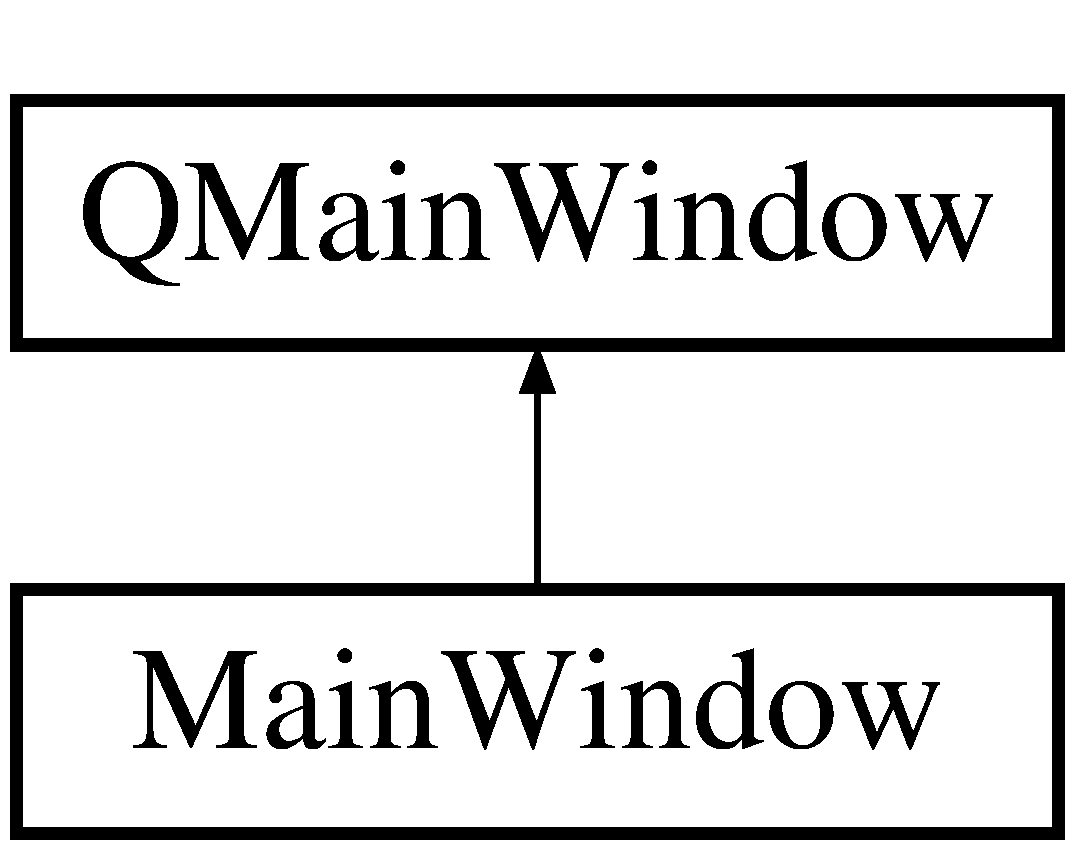
\includegraphics[height=2.000000cm]{class_main_window}
\end{center}
\end{figure}
\subsection*{Public Member Functions}
\begin{DoxyCompactItemize}
\item 
\hypertarget{class_main_window_a8b244be8b7b7db1b08de2a2acb9409db}{}{\bfseries Main\+Window} (Q\+Widget $\ast$parent=0)\label{class_main_window_a8b244be8b7b7db1b08de2a2acb9409db}

\item 
\hypertarget{class_main_window_aff62d9c195294976887758c1598860de}{}Q\+Push\+Button $\ast$ {\bfseries get\+Button\+Show\+Path} () const \label{class_main_window_aff62d9c195294976887758c1598860de}

\item 
\hypertarget{class_main_window_aa5896674ffa88c466f0c8f525c936c3f}{}Q\+Push\+Button $\ast$ {\bfseries get\+Button\+Restart} () const \label{class_main_window_aa5896674ffa88c466f0c8f525c936c3f}

\item 
\hypertarget{class_main_window_a30e41018550c20618efc5acffe4cfb75}{}\hyperlink{class_digital_clock}{Digital\+Clock} $\ast$ {\bfseries get\+Display\+Time} () const \label{class_main_window_a30e41018550c20618efc5acffe4cfb75}

\item 
\hypertarget{class_main_window_a7cb8302f9f923a3f8d4db12b1dfcc6bf}{}Q\+Scroll\+Area $\ast$ {\bfseries get\+View\+Area} () const \label{class_main_window_a7cb8302f9f923a3f8d4db12b1dfcc6bf}

\item 
\hypertarget{class_main_window_a8422d215fa6396b1f8a8bb79540e6002}{}Q\+Label $\ast$ {\bfseries get\+Pontos\+Label} () const \label{class_main_window_a8422d215fa6396b1f8a8bb79540e6002}

\end{DoxyCompactItemize}
\subsection*{Friends}
\begin{DoxyCompactItemize}
\item 
\hypertarget{class_main_window_aa2fab026580d6f14280c2ffb8063a314}{}class {\bfseries Game}\label{class_main_window_aa2fab026580d6f14280c2ffb8063a314}

\end{DoxyCompactItemize}


\subsection{Detailed Description}


Definition at line 24 of file mainwindow.\+h.



The documentation for this class was generated from the following files\+:\begin{DoxyCompactItemize}
\item 
mainwindow.\+h\item 
mainwindow.\+cpp\end{DoxyCompactItemize}

\hypertarget{class_path_finder_a_i}{}\section{Path\+Finder\+A\+I Class Reference}
\label{class_path_finder_a_i}\index{Path\+Finder\+A\+I@{Path\+Finder\+A\+I}}


Cria a inteligencia artificial para caminhar no labirinto ate atingir uma celula. A I\+A foi modelada usando o seguinte\+:  




{\ttfamily \#include $<$pathfinderai.\+h$>$}

Inheritance diagram for Path\+Finder\+A\+I\+:\begin{figure}[H]
\begin{center}
\leavevmode
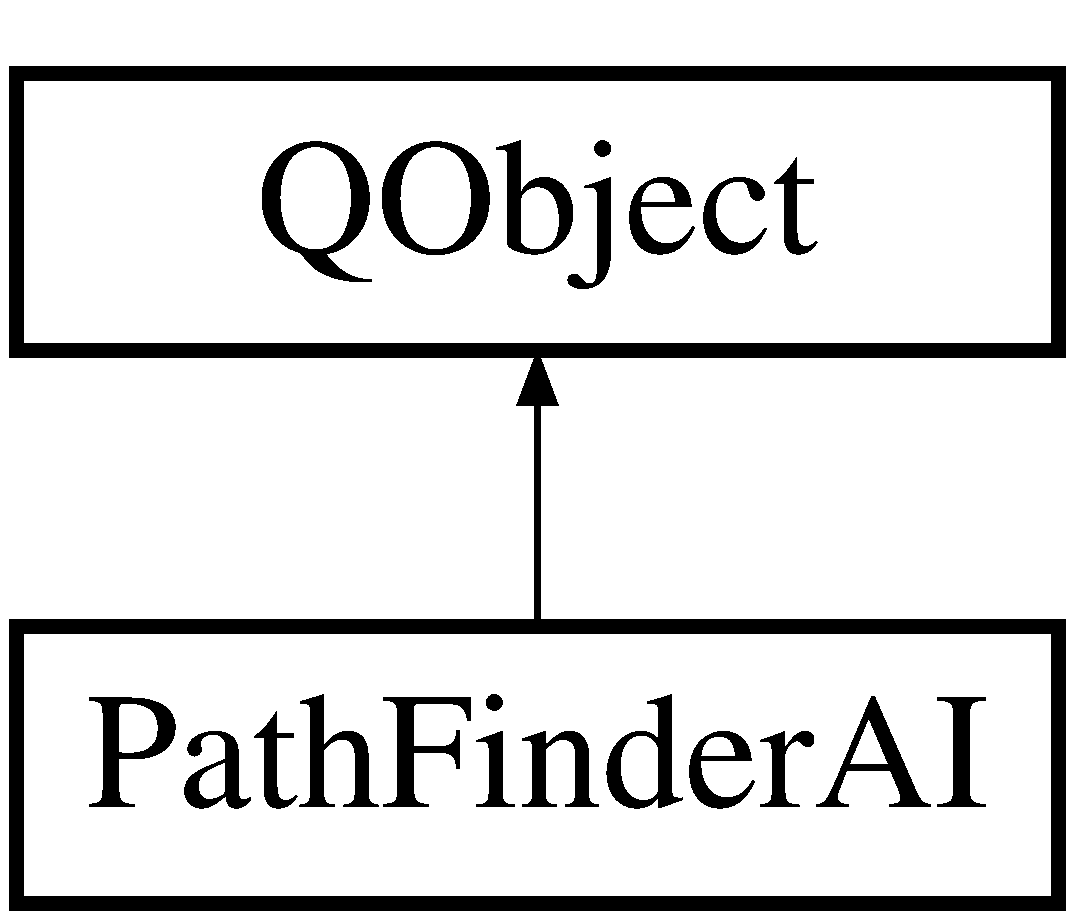
\includegraphics[height=2.000000cm]{class_path_finder_a_i}
\end{center}
\end{figure}
\subsection*{Public Member Functions}
\begin{DoxyCompactItemize}
\item 
bool \hyperlink{class_path_finder_a_i_a2efb996de79146ca2cad3d61d19bd0c9}{start} ()
\begin{DoxyCompactList}\small\item\em Inicia a procura pela celula final. \end{DoxyCompactList}\item 
bool \hyperlink{class_path_finder_a_i_a26b87529dbb30a2c151af42a790e8f61}{stop} ()
\begin{DoxyCompactList}\small\item\em Interrompe a procura pela celula final. \end{DoxyCompactList}\item 
int \hyperlink{class_path_finder_a_i_af3abb07e07360f6e1b60b2b34c38e9e3}{get\+I\+Q} () const 
\begin{DoxyCompactList}\small\item\em Obtem o coeficiente de inteligencia da busca pela celula final. \end{DoxyCompactList}\item 
bool \hyperlink{class_path_finder_a_i_a3e53eb6b981c8721f9670470ea8f4c80}{set\+I\+Q} (int iq)
\begin{DoxyCompactList}\small\item\em Define o coeficiente de inteligencia da busca pela celula final. \end{DoxyCompactList}\item 
\hyperlink{class_labirinto}{Labirinto} $\ast$ \hyperlink{class_path_finder_a_i_aa1634bdbad590e159bcacd43d1a18468}{get\+Labirinto} () const 
\begin{DoxyCompactList}\small\item\em Obtem o labirinto usado na busca. \end{DoxyCompactList}\item 
void \hyperlink{class_path_finder_a_i_a2296c35be51fd6fdc6dd98bf6c344867}{set\+Labirinto} (\hyperlink{class_labirinto}{Labirinto} $\ast$labirinto)
\begin{DoxyCompactList}\small\item\em Define o labirinto usado na busca. \end{DoxyCompactList}\item 
\hyperlink{struct_labirinto_1_1_cell}{Labirinto\+::\+Cell} \hyperlink{class_path_finder_a_i_a7fe151b032792b40f7d2fa9acd33a01c}{get\+Initial\+Cell} () const 
\begin{DoxyCompactList}\small\item\em Obtem a celula inicial, ou seja, aquela da qual comecara a busca. \end{DoxyCompactList}\item 
\hyperlink{struct_labirinto_1_1_cell}{Labirinto\+::\+Cell} \hyperlink{class_path_finder_a_i_a5489d2faf1c7c3f7cdb401d4624231cf}{get\+Final\+Cell} () const 
\begin{DoxyCompactList}\small\item\em Obtem a celula final, ou seja, aquela na qual terminara a busca. \end{DoxyCompactList}\item 
\hyperlink{struct_labirinto_1_1_cell}{Labirinto\+::\+Cell} \hyperlink{class_path_finder_a_i_add2b9e88e3bd509b837b12297c846f10}{get\+Current\+Cell} ()
\begin{DoxyCompactList}\small\item\em Obtem a celula atual na busca. \end{DoxyCompactList}\item 
void \hyperlink{class_path_finder_a_i_aa95d25fd460d4e12fdaf90e8a8715fc4}{set\+Initial\+Cell} (const \hyperlink{struct_labirinto_1_1_cell}{Labirinto\+::\+Cell} \&cell)
\begin{DoxyCompactList}\small\item\em Define a celula inicial. \end{DoxyCompactList}\item 
void \hyperlink{class_path_finder_a_i_a705c39f6d8596d658742b40d5f707058}{set\+Final\+Cell} (const \hyperlink{struct_labirinto_1_1_cell}{Labirinto\+::\+Cell} \&cell)
\begin{DoxyCompactList}\small\item\em Define a celula final. \end{DoxyCompactList}\item 
void \hyperlink{class_path_finder_a_i_ae8ddaab163d826e91c4893d573c4f302}{set\+Current\+Cell} (const \hyperlink{struct_labirinto_1_1_cell}{Labirinto\+::\+Cell} \&cell)
\begin{DoxyCompactList}\small\item\em Define a celula atual. \end{DoxyCompactList}\end{DoxyCompactItemize}


\subsection{Detailed Description}
Cria a inteligencia artificial para caminhar no labirinto ate atingir uma celula. A I\+A foi modelada usando o seguinte\+: 

Projeto\+: Maze Versao\+: 1.\+0b Autores\+: Leno Raimundo
\begin{DoxyItemize}
\item Tempo para tomar uma decisao, ou seja, o tempo para ir para a proxima celula;
\item Probabilidade de tomar a decisao certa, ou seja, a probabilidade de a proxima celula ser a certa;
\item Capacidade de memoria\+: quantidade de celulas ja visitadas que a A\+I consegue lembrar 
\end{DoxyItemize}

Definition at line 27 of file pathfinderai.\+h.



\subsection{Member Function Documentation}
\hypertarget{class_path_finder_a_i_add2b9e88e3bd509b837b12297c846f10}{}\index{Path\+Finder\+A\+I@{Path\+Finder\+A\+I}!get\+Current\+Cell@{get\+Current\+Cell}}
\index{get\+Current\+Cell@{get\+Current\+Cell}!Path\+Finder\+A\+I@{Path\+Finder\+A\+I}}
\subsubsection[{get\+Current\+Cell}]{\setlength{\rightskip}{0pt plus 5cm}{\bf Labirinto\+::\+Cell} Path\+Finder\+A\+I\+::get\+Current\+Cell (
\begin{DoxyParamCaption}
{}
\end{DoxyParamCaption}
)}\label{class_path_finder_a_i_add2b9e88e3bd509b837b12297c846f10}


Obtem a celula atual na busca. 

\begin{DoxyReturn}{Returns}
a celula atual 
\end{DoxyReturn}


Definition at line 38 of file pathfinderai.\+cpp.

\hypertarget{class_path_finder_a_i_a5489d2faf1c7c3f7cdb401d4624231cf}{}\index{Path\+Finder\+A\+I@{Path\+Finder\+A\+I}!get\+Final\+Cell@{get\+Final\+Cell}}
\index{get\+Final\+Cell@{get\+Final\+Cell}!Path\+Finder\+A\+I@{Path\+Finder\+A\+I}}
\subsubsection[{get\+Final\+Cell}]{\setlength{\rightskip}{0pt plus 5cm}{\bf Labirinto\+::\+Cell} Path\+Finder\+A\+I\+::get\+Final\+Cell (
\begin{DoxyParamCaption}
{}
\end{DoxyParamCaption}
) const\hspace{0.3cm}{\ttfamily [inline]}}\label{class_path_finder_a_i_a5489d2faf1c7c3f7cdb401d4624231cf}


Obtem a celula final, ou seja, aquela na qual terminara a busca. 

\begin{DoxyReturn}{Returns}
a celula final 
\end{DoxyReturn}


Definition at line 86 of file pathfinderai.\+h.

\hypertarget{class_path_finder_a_i_a7fe151b032792b40f7d2fa9acd33a01c}{}\index{Path\+Finder\+A\+I@{Path\+Finder\+A\+I}!get\+Initial\+Cell@{get\+Initial\+Cell}}
\index{get\+Initial\+Cell@{get\+Initial\+Cell}!Path\+Finder\+A\+I@{Path\+Finder\+A\+I}}
\subsubsection[{get\+Initial\+Cell}]{\setlength{\rightskip}{0pt plus 5cm}{\bf Labirinto\+::\+Cell} Path\+Finder\+A\+I\+::get\+Initial\+Cell (
\begin{DoxyParamCaption}
{}
\end{DoxyParamCaption}
) const\hspace{0.3cm}{\ttfamily [inline]}}\label{class_path_finder_a_i_a7fe151b032792b40f7d2fa9acd33a01c}


Obtem a celula inicial, ou seja, aquela da qual comecara a busca. 

\begin{DoxyReturn}{Returns}
a celula inicial 
\end{DoxyReturn}


Definition at line 80 of file pathfinderai.\+h.

\hypertarget{class_path_finder_a_i_af3abb07e07360f6e1b60b2b34c38e9e3}{}\index{Path\+Finder\+A\+I@{Path\+Finder\+A\+I}!get\+I\+Q@{get\+I\+Q}}
\index{get\+I\+Q@{get\+I\+Q}!Path\+Finder\+A\+I@{Path\+Finder\+A\+I}}
\subsubsection[{get\+I\+Q}]{\setlength{\rightskip}{0pt plus 5cm}int Path\+Finder\+A\+I\+::get\+I\+Q (
\begin{DoxyParamCaption}
{}
\end{DoxyParamCaption}
) const\hspace{0.3cm}{\ttfamily [inline]}}\label{class_path_finder_a_i_af3abb07e07360f6e1b60b2b34c38e9e3}


Obtem o coeficiente de inteligencia da busca pela celula final. 

\begin{DoxyReturn}{Returns}
um inteiro de 1 a 200 que representa o coeficiente de inteligencia usado na busca 
\end{DoxyReturn}


Definition at line 53 of file pathfinderai.\+h.

\hypertarget{class_path_finder_a_i_aa1634bdbad590e159bcacd43d1a18468}{}\index{Path\+Finder\+A\+I@{Path\+Finder\+A\+I}!get\+Labirinto@{get\+Labirinto}}
\index{get\+Labirinto@{get\+Labirinto}!Path\+Finder\+A\+I@{Path\+Finder\+A\+I}}
\subsubsection[{get\+Labirinto}]{\setlength{\rightskip}{0pt plus 5cm}{\bf Labirinto}$\ast$ Path\+Finder\+A\+I\+::get\+Labirinto (
\begin{DoxyParamCaption}
{}
\end{DoxyParamCaption}
) const\hspace{0.3cm}{\ttfamily [inline]}}\label{class_path_finder_a_i_aa1634bdbad590e159bcacd43d1a18468}


Obtem o labirinto usado na busca. 

\begin{DoxyReturn}{Returns}
o labirinto usado na busca, ou N\+U\+L\+L se ele nao existe. 
\end{DoxyReturn}


Definition at line 68 of file pathfinderai.\+h.

\hypertarget{class_path_finder_a_i_ae8ddaab163d826e91c4893d573c4f302}{}\index{Path\+Finder\+A\+I@{Path\+Finder\+A\+I}!set\+Current\+Cell@{set\+Current\+Cell}}
\index{set\+Current\+Cell@{set\+Current\+Cell}!Path\+Finder\+A\+I@{Path\+Finder\+A\+I}}
\subsubsection[{set\+Current\+Cell}]{\setlength{\rightskip}{0pt plus 5cm}void Path\+Finder\+A\+I\+::set\+Current\+Cell (
\begin{DoxyParamCaption}
\item[{const {\bf Labirinto\+::\+Cell} \&}]{cell}
\end{DoxyParamCaption}
)\hspace{0.3cm}{\ttfamily [inline]}}\label{class_path_finder_a_i_ae8ddaab163d826e91c4893d573c4f302}


Define a celula atual. 


\begin{DoxyParams}{Parameters}
{\em cell} & uma celula valida \\
\hline
\end{DoxyParams}


Definition at line 112 of file pathfinderai.\+h.

\hypertarget{class_path_finder_a_i_a705c39f6d8596d658742b40d5f707058}{}\index{Path\+Finder\+A\+I@{Path\+Finder\+A\+I}!set\+Final\+Cell@{set\+Final\+Cell}}
\index{set\+Final\+Cell@{set\+Final\+Cell}!Path\+Finder\+A\+I@{Path\+Finder\+A\+I}}
\subsubsection[{set\+Final\+Cell}]{\setlength{\rightskip}{0pt plus 5cm}void Path\+Finder\+A\+I\+::set\+Final\+Cell (
\begin{DoxyParamCaption}
\item[{const {\bf Labirinto\+::\+Cell} \&}]{cell}
\end{DoxyParamCaption}
)\hspace{0.3cm}{\ttfamily [inline]}}\label{class_path_finder_a_i_a705c39f6d8596d658742b40d5f707058}


Define a celula final. 


\begin{DoxyParams}{Parameters}
{\em cell} & uma celula valida \\
\hline
\end{DoxyParams}


Definition at line 106 of file pathfinderai.\+h.

\hypertarget{class_path_finder_a_i_aa95d25fd460d4e12fdaf90e8a8715fc4}{}\index{Path\+Finder\+A\+I@{Path\+Finder\+A\+I}!set\+Initial\+Cell@{set\+Initial\+Cell}}
\index{set\+Initial\+Cell@{set\+Initial\+Cell}!Path\+Finder\+A\+I@{Path\+Finder\+A\+I}}
\subsubsection[{set\+Initial\+Cell}]{\setlength{\rightskip}{0pt plus 5cm}void Path\+Finder\+A\+I\+::set\+Initial\+Cell (
\begin{DoxyParamCaption}
\item[{const {\bf Labirinto\+::\+Cell} \&}]{cell}
\end{DoxyParamCaption}
)\hspace{0.3cm}{\ttfamily [inline]}}\label{class_path_finder_a_i_aa95d25fd460d4e12fdaf90e8a8715fc4}


Define a celula inicial. 


\begin{DoxyParams}{Parameters}
{\em cell} & uma celula valida \\
\hline
\end{DoxyParams}


Definition at line 100 of file pathfinderai.\+h.

\hypertarget{class_path_finder_a_i_a3e53eb6b981c8721f9670470ea8f4c80}{}\index{Path\+Finder\+A\+I@{Path\+Finder\+A\+I}!set\+I\+Q@{set\+I\+Q}}
\index{set\+I\+Q@{set\+I\+Q}!Path\+Finder\+A\+I@{Path\+Finder\+A\+I}}
\subsubsection[{set\+I\+Q}]{\setlength{\rightskip}{0pt plus 5cm}bool Path\+Finder\+A\+I\+::set\+I\+Q (
\begin{DoxyParamCaption}
\item[{int}]{iq}
\end{DoxyParamCaption}
)}\label{class_path_finder_a_i_a3e53eb6b981c8721f9670470ea8f4c80}


Define o coeficiente de inteligencia da busca pela celula final. 


\begin{DoxyParams}{Parameters}
{\em iq} & um numero de 1 a 200. Quanto maior, mais rapida e eficiente e a busca pela celula final. \\
\hline
\end{DoxyParams}
\begin{DoxyReturn}{Returns}
sempre true. 
\end{DoxyReturn}


Definition at line 26 of file pathfinderai.\+cpp.

\hypertarget{class_path_finder_a_i_a2296c35be51fd6fdc6dd98bf6c344867}{}\index{Path\+Finder\+A\+I@{Path\+Finder\+A\+I}!set\+Labirinto@{set\+Labirinto}}
\index{set\+Labirinto@{set\+Labirinto}!Path\+Finder\+A\+I@{Path\+Finder\+A\+I}}
\subsubsection[{set\+Labirinto}]{\setlength{\rightskip}{0pt plus 5cm}void Path\+Finder\+A\+I\+::set\+Labirinto (
\begin{DoxyParamCaption}
\item[{{\bf Labirinto} $\ast$}]{labirinto}
\end{DoxyParamCaption}
)\hspace{0.3cm}{\ttfamily [inline]}}\label{class_path_finder_a_i_a2296c35be51fd6fdc6dd98bf6c344867}


Define o labirinto usado na busca. 


\begin{DoxyParams}{Parameters}
{\em labirinto} & um labirinto \\
\hline
\end{DoxyParams}


Definition at line 74 of file pathfinderai.\+h.

\hypertarget{class_path_finder_a_i_a2efb996de79146ca2cad3d61d19bd0c9}{}\index{Path\+Finder\+A\+I@{Path\+Finder\+A\+I}!start@{start}}
\index{start@{start}!Path\+Finder\+A\+I@{Path\+Finder\+A\+I}}
\subsubsection[{start}]{\setlength{\rightskip}{0pt plus 5cm}bool Path\+Finder\+A\+I\+::start (
\begin{DoxyParamCaption}
{}
\end{DoxyParamCaption}
)}\label{class_path_finder_a_i_a2efb996de79146ca2cad3d61d19bd0c9}


Inicia a procura pela celula final. 

\begin{DoxyReturn}{Returns}
sempre true. 
\end{DoxyReturn}


Definition at line 58 of file pathfinderai.\+cpp.

\hypertarget{class_path_finder_a_i_a26b87529dbb30a2c151af42a790e8f61}{}\index{Path\+Finder\+A\+I@{Path\+Finder\+A\+I}!stop@{stop}}
\index{stop@{stop}!Path\+Finder\+A\+I@{Path\+Finder\+A\+I}}
\subsubsection[{stop}]{\setlength{\rightskip}{0pt plus 5cm}bool Path\+Finder\+A\+I\+::stop (
\begin{DoxyParamCaption}
{}
\end{DoxyParamCaption}
)}\label{class_path_finder_a_i_a26b87529dbb30a2c151af42a790e8f61}


Interrompe a procura pela celula final. 

\begin{DoxyReturn}{Returns}
sempre true. 
\end{DoxyReturn}


Definition at line 18 of file pathfinderai.\+cpp.



The documentation for this class was generated from the following files\+:\begin{DoxyCompactItemize}
\item 
pathfinderai.\+h\item 
pathfinderai.\+cpp\end{DoxyCompactItemize}

\hypertarget{class_player}{}\section{Player Class Reference}
\label{class_player}\index{Player@{Player}}


Representa um jogador.  




{\ttfamily \#include $<$player.\+h$>$}

\subsection*{Public Member Functions}
\begin{DoxyCompactItemize}
\item 
\hypertarget{class_player_a32aad167b7d41694952c3731c5e55ea4}{}{\bfseries Player} (const std\+::string \&name=\char`\"{}Sem nome\char`\"{}, const \hyperlink{class_color}{Color} \&color=\hyperlink{class_color}{Color}(255, 0, 0))\label{class_player_a32aad167b7d41694952c3731c5e55ea4}

\item 
\hyperlink{struct_labirinto_1_1_cell}{Labirinto\+::\+Cell} \hyperlink{class_player_ac080f98d0b6ab04f07e2e2e65868c11c}{get\+Cell} () const 
\begin{DoxyCompactList}\small\item\em Obtem a celula na qual o jogador esta. \end{DoxyCompactList}\item 
bool \hyperlink{class_player_a7b7a8bf62f14126e4b8baf8ef087ac97}{set\+Cell} (const \hyperlink{struct_labirinto_1_1_cell}{Labirinto\+::\+Cell} \&cell)
\begin{DoxyCompactList}\small\item\em Define a celula na qual o jogador esta. \end{DoxyCompactList}\item 
\hypertarget{class_player_a3660536cb21311d5480df9a2dc8b051a}{}\hyperlink{class_color}{Color} {\bfseries get\+Color} () const \label{class_player_a3660536cb21311d5480df9a2dc8b051a}

\item 
\hypertarget{class_player_a647e6a411f2fb94dce137307a5d9785e}{}void {\bfseries set\+Color} (const \hyperlink{class_color}{Color} \&color)\label{class_player_a647e6a411f2fb94dce137307a5d9785e}

\end{DoxyCompactItemize}


\subsection{Detailed Description}
Representa um jogador. 

Projeto\+: Maze Versao\+: 1.\+0b Autores\+: Leno Raimundo 

Definition at line 21 of file player.\+h.



\subsection{Member Function Documentation}
\hypertarget{class_player_ac080f98d0b6ab04f07e2e2e65868c11c}{}\index{Player@{Player}!get\+Cell@{get\+Cell}}
\index{get\+Cell@{get\+Cell}!Player@{Player}}
\subsubsection[{get\+Cell}]{\setlength{\rightskip}{0pt plus 5cm}{\bf Labirinto\+::\+Cell} Player\+::get\+Cell (
\begin{DoxyParamCaption}
{}
\end{DoxyParamCaption}
) const\hspace{0.3cm}{\ttfamily [inline]}}\label{class_player_ac080f98d0b6ab04f07e2e2e65868c11c}


Obtem a celula na qual o jogador esta. 

\begin{DoxyReturn}{Returns}
a celula na qual o jogador esta 
\end{DoxyReturn}


Definition at line 32 of file player.\+h.

\hypertarget{class_player_a7b7a8bf62f14126e4b8baf8ef087ac97}{}\index{Player@{Player}!set\+Cell@{set\+Cell}}
\index{set\+Cell@{set\+Cell}!Player@{Player}}
\subsubsection[{set\+Cell}]{\setlength{\rightskip}{0pt plus 5cm}bool Player\+::set\+Cell (
\begin{DoxyParamCaption}
\item[{const {\bf Labirinto\+::\+Cell} \&}]{cell}
\end{DoxyParamCaption}
)}\label{class_player_a7b7a8bf62f14126e4b8baf8ef087ac97}


Define a celula na qual o jogador esta. 


\begin{DoxyParams}{Parameters}
{\em cell} & uma celua valida \\
\hline
\end{DoxyParams}
\begin{DoxyReturn}{Returns}
true. 
\end{DoxyReturn}


Definition at line 22 of file player.\+cpp.



The documentation for this class was generated from the following files\+:\begin{DoxyCompactItemize}
\item 
player.\+h\item 
player.\+cpp\end{DoxyCompactItemize}

\hypertarget{class_queue}{}\section{Queue$<$ T\+Y\+P\+E $>$ Class Template Reference}
\label{class_queue}\index{Queue$<$ T\+Y\+P\+E $>$@{Queue$<$ T\+Y\+P\+E $>$}}
\subsection*{Public Member Functions}
\begin{DoxyCompactItemize}
\item 
\hyperlink{class_queue_a2da5c01a70e99abfedf529f2592fa55c}{Queue} ()
\item 
\hyperlink{class_queue_acc8135c39b42b208a665bbc96e56b663}{$\sim$\+Queue} ()
\item 
T\+Y\+P\+E \hyperlink{class_queue_a0a47859a45541aec9192c26a44055445}{front} ()
\item 
bool \hyperlink{class_queue_af0d8e729c853a5d56b275260b3c63565}{enqueue} (T\+Y\+P\+E value)
\item 
T\+Y\+P\+E \hyperlink{class_queue_ae76570adc4adad92792440083a58d594}{dequeue} ()
\item 
bool \hyperlink{class_queue_a48881097f65860e871b4bd7469f0ba8f}{is\+Empty} ()
\item 
void \hyperlink{class_queue_ac6c6e763f72fa7c0556ad29005fdafd7}{print} ()
\end{DoxyCompactItemize}


\subsection{Detailed Description}
\subsubsection*{template$<$typename T\+Y\+P\+E$>$class Queue$<$ T\+Y\+P\+E $>$}



Definition at line 6 of file queue.\+h.



\subsection{Constructor \& Destructor Documentation}
\hypertarget{class_queue_a2da5c01a70e99abfedf529f2592fa55c}{}\index{Queue@{Queue}!Queue@{Queue}}
\index{Queue@{Queue}!Queue@{Queue}}
\subsubsection[{Queue}]{\setlength{\rightskip}{0pt plus 5cm}template$<$typename T\+Y\+P\+E $>$ {\bf Queue}$<$ T\+Y\+P\+E $>$\+::{\bf Queue} (
\begin{DoxyParamCaption}
{}
\end{DoxyParamCaption}
)\hspace{0.3cm}{\ttfamily [inline]}}\label{class_queue_a2da5c01a70e99abfedf529f2592fa55c}
Descrição\+: Metodo construtor.

Parâmetros\+: Não possui.

\begin{DoxyReturn}{Returns}
. 
\end{DoxyReturn}


Definition at line 16 of file queue.\+h.

\hypertarget{class_queue_acc8135c39b42b208a665bbc96e56b663}{}\index{Queue@{Queue}!````~Queue@{$\sim$\+Queue}}
\index{````~Queue@{$\sim$\+Queue}!Queue@{Queue}}
\subsubsection[{$\sim$\+Queue}]{\setlength{\rightskip}{0pt plus 5cm}template$<$typename T\+Y\+P\+E $>$ {\bf Queue}$<$ T\+Y\+P\+E $>$\+::$\sim${\bf Queue} (
\begin{DoxyParamCaption}
{}
\end{DoxyParamCaption}
)\hspace{0.3cm}{\ttfamily [inline]}}\label{class_queue_acc8135c39b42b208a665bbc96e56b663}
Descrição\+: Metodo destrutor

Parâmetros\+: Não possui.

\begin{DoxyReturn}{Returns}
. 
\end{DoxyReturn}


Definition at line 25 of file queue.\+h.



\subsection{Member Function Documentation}
\hypertarget{class_queue_ae76570adc4adad92792440083a58d594}{}\index{Queue@{Queue}!dequeue@{dequeue}}
\index{dequeue@{dequeue}!Queue@{Queue}}
\subsubsection[{dequeue}]{\setlength{\rightskip}{0pt plus 5cm}template$<$typename T\+Y\+P\+E $>$ T\+Y\+P\+E {\bf Queue}$<$ T\+Y\+P\+E $>$\+::dequeue (
\begin{DoxyParamCaption}
{}
\end{DoxyParamCaption}
)\hspace{0.3cm}{\ttfamily [inline]}}\label{class_queue_ae76570adc4adad92792440083a58d594}
Descrição\+: Metodo responsável por remover o primeiro elemento da fila.

Parâmetros\+: Não possui.

\begin{DoxyReturn}{Returns}
T\+Y\+P\+E. valor retornado\+: O valor do elemento removido. 
\end{DoxyReturn}


Definition at line 61 of file queue.\+h.

\hypertarget{class_queue_af0d8e729c853a5d56b275260b3c63565}{}\index{Queue@{Queue}!enqueue@{enqueue}}
\index{enqueue@{enqueue}!Queue@{Queue}}
\subsubsection[{enqueue}]{\setlength{\rightskip}{0pt plus 5cm}template$<$typename T\+Y\+P\+E $>$ bool {\bf Queue}$<$ T\+Y\+P\+E $>$\+::enqueue (
\begin{DoxyParamCaption}
\item[{T\+Y\+P\+E}]{value}
\end{DoxyParamCaption}
)\hspace{0.3cm}{\ttfamily [inline]}}\label{class_queue_af0d8e729c853a5d56b275260b3c63565}
Descrição\+: Metodo responsável por adicionar o ultimo elemento da fila.

Parâmetros\+: value(o valor a ser adicionado).

\begin{DoxyReturn}{Returns}
bool. valor retornado\+: Verdadeiro se o elemento foi adicionado ou falso caso contrário (memória cheia, por exemplo). 
\end{DoxyReturn}


Definition at line 48 of file queue.\+h.

\hypertarget{class_queue_a0a47859a45541aec9192c26a44055445}{}\index{Queue@{Queue}!front@{front}}
\index{front@{front}!Queue@{Queue}}
\subsubsection[{front}]{\setlength{\rightskip}{0pt plus 5cm}template$<$typename T\+Y\+P\+E $>$ T\+Y\+P\+E {\bf Queue}$<$ T\+Y\+P\+E $>$\+::front (
\begin{DoxyParamCaption}
{}
\end{DoxyParamCaption}
)\hspace{0.3cm}{\ttfamily [inline]}}\label{class_queue_a0a47859a45541aec9192c26a44055445}
Descrição\+: Metodo responsável por pegar o primeiro elemento da fila.

Parâmetros\+: Não possui.

\begin{DoxyReturn}{Returns}
T\+Y\+P\+E. valor retornado\+: Retorna o primeiro elemento da fila. 
\end{DoxyReturn}


Definition at line 35 of file queue.\+h.

\hypertarget{class_queue_a48881097f65860e871b4bd7469f0ba8f}{}\index{Queue@{Queue}!is\+Empty@{is\+Empty}}
\index{is\+Empty@{is\+Empty}!Queue@{Queue}}
\subsubsection[{is\+Empty}]{\setlength{\rightskip}{0pt plus 5cm}template$<$typename T\+Y\+P\+E $>$ bool {\bf Queue}$<$ T\+Y\+P\+E $>$\+::is\+Empty (
\begin{DoxyParamCaption}
{}
\end{DoxyParamCaption}
)\hspace{0.3cm}{\ttfamily [inline]}}\label{class_queue_a48881097f65860e871b4bd7469f0ba8f}
Descrição\+: Metodo responsável por verficar se existe elemento da fila.

Parâmetros\+: Não possui.

\begin{DoxyReturn}{Returns}
bool. valor retornado\+: Se não possui elemento retorna true, se possui retorna false. 
\end{DoxyReturn}


Definition at line 74 of file queue.\+h.

\hypertarget{class_queue_ac6c6e763f72fa7c0556ad29005fdafd7}{}\index{Queue@{Queue}!print@{print}}
\index{print@{print}!Queue@{Queue}}
\subsubsection[{print}]{\setlength{\rightskip}{0pt plus 5cm}template$<$typename T\+Y\+P\+E $>$ void {\bf Queue}$<$ T\+Y\+P\+E $>$\+::print (
\begin{DoxyParamCaption}
{}
\end{DoxyParamCaption}
)\hspace{0.3cm}{\ttfamily [inline]}}\label{class_queue_ac6c6e763f72fa7c0556ad29005fdafd7}
Descrição\+: Metodo responsável por imprimir os elementos da fila.

Parâmetros\+: Não possui.

\begin{DoxyReturn}{Returns}
void. 
\end{DoxyReturn}


Definition at line 86 of file queue.\+h.



The documentation for this class was generated from the following file\+:\begin{DoxyCompactItemize}
\item 
queue.\+h\end{DoxyCompactItemize}

\hypertarget{struct_game_1_1_rank}{}\section{Game\+:\+:Rank Struct Reference}
\label{struct_game_1_1_rank}\index{Game\+::\+Rank@{Game\+::\+Rank}}
\subsection*{Public Attributes}
\begin{DoxyCompactItemize}
\item 
\hypertarget{struct_game_1_1_rank_a96ed516eff0de27b59eb22284c34cb6d}{}std\+::string {\bfseries nome}\label{struct_game_1_1_rank_a96ed516eff0de27b59eb22284c34cb6d}

\item 
\hypertarget{struct_game_1_1_rank_afa37c13c67a922ace2e342aadee5a4e4}{}int {\bfseries pontos} = 0\label{struct_game_1_1_rank_afa37c13c67a922ace2e342aadee5a4e4}

\end{DoxyCompactItemize}


\subsection{Detailed Description}


Definition at line 57 of file game.\+h.



The documentation for this struct was generated from the following file\+:\begin{DoxyCompactItemize}
\item 
game.\+h\end{DoxyCompactItemize}

\hypertarget{class_rect}{}\section{Rect Class Reference}
\label{class_rect}\index{Rect@{Rect}}


Define um retangulo.  




{\ttfamily \#include $<$rect.\+h$>$}

\subsection*{Public Member Functions}
\begin{DoxyCompactItemize}
\item 
\hypertarget{class_rect_a5b9c0acb135c198ca69354a67bf7e054}{}{\bfseries Rect} (int x1=0, int y1=0, int w1=0, int h1=0)\label{class_rect_a5b9c0acb135c198ca69354a67bf7e054}

\end{DoxyCompactItemize}
\subsection*{Public Attributes}
\begin{DoxyCompactItemize}
\item 
\hypertarget{class_rect_a64d1ef14e429e1816539de4c54361e55}{}int {\bfseries x}\label{class_rect_a64d1ef14e429e1816539de4c54361e55}

\item 
\hypertarget{class_rect_a1e37b6f8a4fb0d68ba22c8fffffab0a4}{}int {\bfseries y}\label{class_rect_a1e37b6f8a4fb0d68ba22c8fffffab0a4}

\item 
\hypertarget{class_rect_a36b6c8bb15c7706c3b2b3e91345e11f8}{}int {\bfseries w}\label{class_rect_a36b6c8bb15c7706c3b2b3e91345e11f8}

\item 
\hypertarget{class_rect_af9111a21106ba65952da60320ea91df6}{}int {\bfseries h}\label{class_rect_af9111a21106ba65952da60320ea91df6}

\end{DoxyCompactItemize}


\subsection{Detailed Description}
Define um retangulo. 

Projeto\+: Maze Versao\+: 1.\+0b Autores\+: Leno Raimundo 

Definition at line 14 of file rect.\+h.



The documentation for this class was generated from the following file\+:\begin{DoxyCompactItemize}
\item 
rect.\+h\end{DoxyCompactItemize}

\hypertarget{class_sequence}{}\section{Sequence$<$ T\+Y\+P\+E $>$ Class Template Reference}
\label{class_sequence}\index{Sequence$<$ T\+Y\+P\+E $>$@{Sequence$<$ T\+Y\+P\+E $>$}}
\subsection*{Public Member Functions}
\begin{DoxyCompactItemize}
\item 
\hyperlink{class_sequence_a69865d17cd69ba765a6cb034be7539b9}{Sequence} ()
\item 
\hyperlink{class_sequence_ace9aa11de35439018052db2efb8a7369}{$\sim$\+Sequence} ()
\item 
\hyperlink{class_sequence_a73d0aa763847bbaa3b2d4eca62abc8f7}{Sequence} (const \hyperlink{class_sequence}{Sequence}$<$ T\+Y\+P\+E $>$ \&s)
\item 
bool \hyperlink{class_sequence_a6418341e58be9f5d8303266521f5b4d3}{is\+Empty} ()
\item 
int \hyperlink{class_sequence_aa10151201b866f031d800519c94b1f60}{get\+Size} ()
\item 
bool \hyperlink{class_sequence_a4cc033f7279c21353908bc322985450d}{add\+First} (const T\+Y\+P\+E \&value)
\item 
bool \hyperlink{class_sequence_aba18baeedbc81a9b24c9331b4ee78881}{add\+Last} (const T\+Y\+P\+E \&value)
\item 
bool \hyperlink{class_sequence_a5c9bdbf02bea5ef4552c127f8bc40bda}{add} (const T\+Y\+P\+E \&value, int pos=0)
\item 
T\+Y\+P\+E \hyperlink{class_sequence_a6c2f27cca357a3f494e7f05209f11afc}{remove\+First} ()
\item 
T\+Y\+P\+E \hyperlink{class_sequence_a5325f9adedf34e7bbbae9a5241b167b0}{remove\+Last} ()
\item 
T\+Y\+P\+E \hyperlink{class_sequence_a041bb764297bfb85fe76a3fe21f80533}{remove} (int pos=0)
\item 
T\+Y\+P\+E \hyperlink{class_sequence_ac53c75e455dc23747148bbc14f808a91}{get\+First} ()
\item 
T\+Y\+P\+E \hyperlink{class_sequence_a25eacb0919853eab899ff5c687a0a26a}{get\+Last} ()
\item 
T\+Y\+P\+E \hyperlink{class_sequence_a08130d1d69774ffbe0f8942121604b12}{get} (int pos=0)
\item 
int \hyperlink{class_sequence_a52d217525d72abdca19e52c5f287734c}{search} (const T\+Y\+P\+E \&elm)
\item 
bool \hyperlink{class_sequence_ae9b4b08e48aa47199a1db42dd983c294}{is\+Equal} (\hyperlink{class_sequence}{Sequence}$<$ T\+Y\+P\+E $>$ \&s)
\item 
void \hyperlink{class_sequence_a377edb6182dd993d65d294f300033c19}{reverse} ()
\item 
void \hyperlink{class_sequence_a7c506a0479ef801d45871a81a1804e26}{sort} ()
\item 
void \hyperlink{class_sequence_aa60f1dca0a449df7bf830eab4a243742}{print} ()
\end{DoxyCompactItemize}
\subsection*{Public Attributes}
\begin{DoxyCompactItemize}
\item 
\hypertarget{class_sequence_a98514e1ef695d598b4ebc5b6ca1cb350}{}Node {\bfseries list}\label{class_sequence_a98514e1ef695d598b4ebc5b6ca1cb350}

\end{DoxyCompactItemize}


\subsection{Detailed Description}
\subsubsection*{template$<$typename T\+Y\+P\+E$>$class Sequence$<$ T\+Y\+P\+E $>$}



Definition at line 9 of file sequence.\+h.



\subsection{Constructor \& Destructor Documentation}
\hypertarget{class_sequence_a69865d17cd69ba765a6cb034be7539b9}{}\index{Sequence@{Sequence}!Sequence@{Sequence}}
\index{Sequence@{Sequence}!Sequence@{Sequence}}
\subsubsection[{Sequence}]{\setlength{\rightskip}{0pt plus 5cm}template$<$typename T\+Y\+P\+E $>$ {\bf Sequence}$<$ T\+Y\+P\+E $>$\+::{\bf Sequence} (
\begin{DoxyParamCaption}
{}
\end{DoxyParamCaption}
)}\label{class_sequence_a69865d17cd69ba765a6cb034be7539b9}
Inicializa a sequência 

Definition at line 3 of file sequence.\+cpp.

\hypertarget{class_sequence_ace9aa11de35439018052db2efb8a7369}{}\index{Sequence@{Sequence}!````~Sequence@{$\sim$\+Sequence}}
\index{````~Sequence@{$\sim$\+Sequence}!Sequence@{Sequence}}
\subsubsection[{$\sim$\+Sequence}]{\setlength{\rightskip}{0pt plus 5cm}template$<$typename T\+Y\+P\+E $>$ {\bf Sequence}$<$ T\+Y\+P\+E $>$\+::$\sim${\bf Sequence} (
\begin{DoxyParamCaption}
{}
\end{DoxyParamCaption}
)}\label{class_sequence_ace9aa11de35439018052db2efb8a7369}
Desaloca todos os elementos da sequência e volta ao estado inicial 

Definition at line 6 of file sequence.\+cpp.

\hypertarget{class_sequence_a73d0aa763847bbaa3b2d4eca62abc8f7}{}\index{Sequence@{Sequence}!Sequence@{Sequence}}
\index{Sequence@{Sequence}!Sequence@{Sequence}}
\subsubsection[{Sequence}]{\setlength{\rightskip}{0pt plus 5cm}template$<$typename T\+Y\+P\+E$>$ {\bf Sequence}$<$ T\+Y\+P\+E $>$\+::{\bf Sequence} (
\begin{DoxyParamCaption}
\item[{const {\bf Sequence}$<$ T\+Y\+P\+E $>$ \&}]{s}
\end{DoxyParamCaption}
)}\label{class_sequence_a73d0aa763847bbaa3b2d4eca62abc8f7}
Constrói uma nova sequência a partir de uma já existente (os dados são duplicados) 

\subsection{Member Function Documentation}
\hypertarget{class_sequence_a5c9bdbf02bea5ef4552c127f8bc40bda}{}\index{Sequence@{Sequence}!add@{add}}
\index{add@{add}!Sequence@{Sequence}}
\subsubsection[{add}]{\setlength{\rightskip}{0pt plus 5cm}template$<$typename T\+Y\+P\+E $>$ bool {\bf Sequence}$<$ T\+Y\+P\+E $>$\+::add (
\begin{DoxyParamCaption}
\item[{const T\+Y\+P\+E \&}]{value, }
\item[{int}]{pos = {\ttfamily 0}}
\end{DoxyParamCaption}
)}\label{class_sequence_a5c9bdbf02bea5ef4552c127f8bc40bda}
Adiciona um elemento em uma posição específica da sequência. Se a posição dada for negativa, insere no ínicio. Se a posição for maior que o tamanho da sequência, insere no final. 
\begin{DoxyParams}{Parameters}
{\em value} & Elemento a ser inserido \\
\hline
{\em pos} & Posição do elemento a ser inserido \\
\hline
\end{DoxyParams}
\begin{DoxyReturn}{Returns}
Verdadeiro se o elemento foi adicionado ou falso caso contrário (memória cheia, por exemplo) 
\end{DoxyReturn}


Definition at line 84 of file sequence.\+cpp.

\hypertarget{class_sequence_a4cc033f7279c21353908bc322985450d}{}\index{Sequence@{Sequence}!add\+First@{add\+First}}
\index{add\+First@{add\+First}!Sequence@{Sequence}}
\subsubsection[{add\+First}]{\setlength{\rightskip}{0pt plus 5cm}template$<$typename T\+Y\+P\+E $>$ bool {\bf Sequence}$<$ T\+Y\+P\+E $>$\+::add\+First (
\begin{DoxyParamCaption}
\item[{const T\+Y\+P\+E \&}]{value}
\end{DoxyParamCaption}
)}\label{class_sequence_a4cc033f7279c21353908bc322985450d}
Adiciona um elemento no início da sequência. 
\begin{DoxyParams}{Parameters}
{\em value} & Elemento a ser inserido \\
\hline
\end{DoxyParams}
\begin{DoxyReturn}{Returns}
Verdadeiro se o elemento foi adicionado ou falso caso contrário (memória cheia, por exemplo) 
\end{DoxyReturn}


Definition at line 54 of file sequence.\+cpp.

\hypertarget{class_sequence_aba18baeedbc81a9b24c9331b4ee78881}{}\index{Sequence@{Sequence}!add\+Last@{add\+Last}}
\index{add\+Last@{add\+Last}!Sequence@{Sequence}}
\subsubsection[{add\+Last}]{\setlength{\rightskip}{0pt plus 5cm}template$<$typename T\+Y\+P\+E $>$ bool {\bf Sequence}$<$ T\+Y\+P\+E $>$\+::add\+Last (
\begin{DoxyParamCaption}
\item[{const T\+Y\+P\+E \&}]{value}
\end{DoxyParamCaption}
)}\label{class_sequence_aba18baeedbc81a9b24c9331b4ee78881}
Adiciona um elemento no final da sequência 
\begin{DoxyParams}{Parameters}
{\em value} & Elemento a ser inserido \\
\hline
\end{DoxyParams}
\begin{DoxyReturn}{Returns}
Verdadeiro se o elemento foi adicionado ou falso caso contrário (memória cheia, por exemplo) 
\end{DoxyReturn}


Definition at line 69 of file sequence.\+cpp.

\hypertarget{class_sequence_a08130d1d69774ffbe0f8942121604b12}{}\index{Sequence@{Sequence}!get@{get}}
\index{get@{get}!Sequence@{Sequence}}
\subsubsection[{get}]{\setlength{\rightskip}{0pt plus 5cm}template$<$typename T\+Y\+P\+E $>$ T\+Y\+P\+E {\bf Sequence}$<$ T\+Y\+P\+E $>$\+::get (
\begin{DoxyParamCaption}
\item[{int}]{pos = {\ttfamily 0}}
\end{DoxyParamCaption}
)}\label{class_sequence_a08130d1d69774ffbe0f8942121604b12}
Consulta o elemento de uma posição específica \begin{DoxyReturn}{Returns}
Uma cópia do elemento 
\end{DoxyReturn}


Definition at line 194 of file sequence.\+cpp.

\hypertarget{class_sequence_ac53c75e455dc23747148bbc14f808a91}{}\index{Sequence@{Sequence}!get\+First@{get\+First}}
\index{get\+First@{get\+First}!Sequence@{Sequence}}
\subsubsection[{get\+First}]{\setlength{\rightskip}{0pt plus 5cm}template$<$typename T\+Y\+P\+E $>$ T\+Y\+P\+E {\bf Sequence}$<$ T\+Y\+P\+E $>$\+::get\+First (
\begin{DoxyParamCaption}
{}
\end{DoxyParamCaption}
)}\label{class_sequence_ac53c75e455dc23747148bbc14f808a91}
Consulta o primeiro elemento da sequência \begin{DoxyReturn}{Returns}
Uma cópia do primeiro elemento 
\end{DoxyReturn}


Definition at line 182 of file sequence.\+cpp.

\hypertarget{class_sequence_a25eacb0919853eab899ff5c687a0a26a}{}\index{Sequence@{Sequence}!get\+Last@{get\+Last}}
\index{get\+Last@{get\+Last}!Sequence@{Sequence}}
\subsubsection[{get\+Last}]{\setlength{\rightskip}{0pt plus 5cm}template$<$typename T\+Y\+P\+E $>$ T\+Y\+P\+E {\bf Sequence}$<$ T\+Y\+P\+E $>$\+::get\+Last (
\begin{DoxyParamCaption}
{}
\end{DoxyParamCaption}
)}\label{class_sequence_a25eacb0919853eab899ff5c687a0a26a}
Consulta o último elemento da sequência \begin{DoxyReturn}{Returns}
Uma cópia do último elemento 
\end{DoxyReturn}


Definition at line 188 of file sequence.\+cpp.

\hypertarget{class_sequence_aa10151201b866f031d800519c94b1f60}{}\index{Sequence@{Sequence}!get\+Size@{get\+Size}}
\index{get\+Size@{get\+Size}!Sequence@{Sequence}}
\subsubsection[{get\+Size}]{\setlength{\rightskip}{0pt plus 5cm}template$<$typename T\+Y\+P\+E $>$ int {\bf Sequence}$<$ T\+Y\+P\+E $>$\+::get\+Size (
\begin{DoxyParamCaption}
{}
\end{DoxyParamCaption}
)}\label{class_sequence_aa10151201b866f031d800519c94b1f60}
Retorna o número de elementos na sequência 

Definition at line 41 of file sequence.\+cpp.

\hypertarget{class_sequence_a6418341e58be9f5d8303266521f5b4d3}{}\index{Sequence@{Sequence}!is\+Empty@{is\+Empty}}
\index{is\+Empty@{is\+Empty}!Sequence@{Sequence}}
\subsubsection[{is\+Empty}]{\setlength{\rightskip}{0pt plus 5cm}template$<$typename T\+Y\+P\+E $>$ bool {\bf Sequence}$<$ T\+Y\+P\+E $>$\+::is\+Empty (
\begin{DoxyParamCaption}
{}
\end{DoxyParamCaption}
)}\label{class_sequence_a6418341e58be9f5d8303266521f5b4d3}
Verifica se a sequência está vazia \begin{DoxyReturn}{Returns}
se vazia retorna true se não false. 
\end{DoxyReturn}


Definition at line 35 of file sequence.\+cpp.

\hypertarget{class_sequence_ae9b4b08e48aa47199a1db42dd983c294}{}\index{Sequence@{Sequence}!is\+Equal@{is\+Equal}}
\index{is\+Equal@{is\+Equal}!Sequence@{Sequence}}
\subsubsection[{is\+Equal}]{\setlength{\rightskip}{0pt plus 5cm}template$<$typename T\+Y\+P\+E $>$ bool {\bf Sequence}$<$ T\+Y\+P\+E $>$\+::is\+Equal (
\begin{DoxyParamCaption}
\item[{{\bf Sequence}$<$ T\+Y\+P\+E $>$ \&}]{s}
\end{DoxyParamCaption}
)}\label{class_sequence_ae9b4b08e48aa47199a1db42dd983c294}
Verifica se todos os elementos (e sua ordem) de uma sequência são iguais aos elementos de outra sequência 
\begin{DoxyParams}{Parameters}
{\em s} & Sequência a ser comparada \\
\hline
\end{DoxyParams}
\begin{DoxyReturn}{Returns}
Verdadeiro se elas forem iguais ou falso caso contrário 
\end{DoxyReturn}


Definition at line 232 of file sequence.\+cpp.

\hypertarget{class_sequence_aa60f1dca0a449df7bf830eab4a243742}{}\index{Sequence@{Sequence}!print@{print}}
\index{print@{print}!Sequence@{Sequence}}
\subsubsection[{print}]{\setlength{\rightskip}{0pt plus 5cm}template$<$typename T\+Y\+P\+E $>$ void {\bf Sequence}$<$ T\+Y\+P\+E $>$\+::print (
\begin{DoxyParamCaption}
{}
\end{DoxyParamCaption}
)}\label{class_sequence_aa60f1dca0a449df7bf830eab4a243742}
Envia para a saída-\/padrão os elementos da sequência. 

Definition at line 302 of file sequence.\+cpp.

\hypertarget{class_sequence_a041bb764297bfb85fe76a3fe21f80533}{}\index{Sequence@{Sequence}!remove@{remove}}
\index{remove@{remove}!Sequence@{Sequence}}
\subsubsection[{remove}]{\setlength{\rightskip}{0pt plus 5cm}template$<$typename T\+Y\+P\+E $>$ T\+Y\+P\+E {\bf Sequence}$<$ T\+Y\+P\+E $>$\+::remove (
\begin{DoxyParamCaption}
\item[{int}]{pos = {\ttfamily 0}}
\end{DoxyParamCaption}
)}\label{class_sequence_a041bb764297bfb85fe76a3fe21f80533}
Remove o elemento de uma posição específica. Se a posição dada for negativa, remove o primeiro elemento. Se for maior que o tamanho, remove o último. 
\begin{DoxyParams}{Parameters}
{\em pos} & Posição do elemento a ser removido \\
\hline
\end{DoxyParams}
\begin{DoxyReturn}{Returns}
Uma cópia do elemento removido 
\end{DoxyReturn}


Definition at line 150 of file sequence.\+cpp.

\hypertarget{class_sequence_a6c2f27cca357a3f494e7f05209f11afc}{}\index{Sequence@{Sequence}!remove\+First@{remove\+First}}
\index{remove\+First@{remove\+First}!Sequence@{Sequence}}
\subsubsection[{remove\+First}]{\setlength{\rightskip}{0pt plus 5cm}template$<$typename T\+Y\+P\+E $>$ T\+Y\+P\+E {\bf Sequence}$<$ T\+Y\+P\+E $>$\+::remove\+First (
\begin{DoxyParamCaption}
{}
\end{DoxyParamCaption}
)}\label{class_sequence_a6c2f27cca357a3f494e7f05209f11afc}
Remove o primeiro elemento da sequência \begin{DoxyReturn}{Returns}
Uma cópia do elemento removido 
\end{DoxyReturn}


Definition at line 118 of file sequence.\+cpp.

\hypertarget{class_sequence_a5325f9adedf34e7bbbae9a5241b167b0}{}\index{Sequence@{Sequence}!remove\+Last@{remove\+Last}}
\index{remove\+Last@{remove\+Last}!Sequence@{Sequence}}
\subsubsection[{remove\+Last}]{\setlength{\rightskip}{0pt plus 5cm}template$<$typename T\+Y\+P\+E $>$ T\+Y\+P\+E {\bf Sequence}$<$ T\+Y\+P\+E $>$\+::remove\+Last (
\begin{DoxyParamCaption}
{}
\end{DoxyParamCaption}
)}\label{class_sequence_a5325f9adedf34e7bbbae9a5241b167b0}
Remove o último elemento da sequência \begin{DoxyReturn}{Returns}
Uma cópia do elemento removido 
\end{DoxyReturn}


Definition at line 134 of file sequence.\+cpp.

\hypertarget{class_sequence_a377edb6182dd993d65d294f300033c19}{}\index{Sequence@{Sequence}!reverse@{reverse}}
\index{reverse@{reverse}!Sequence@{Sequence}}
\subsubsection[{reverse}]{\setlength{\rightskip}{0pt plus 5cm}template$<$typename T\+Y\+P\+E $>$ void {\bf Sequence}$<$ T\+Y\+P\+E $>$\+::reverse (
\begin{DoxyParamCaption}
{}
\end{DoxyParamCaption}
)}\label{class_sequence_a377edb6182dd993d65d294f300033c19}
Inverte os elementos de uma sequência. O primeiro passa a ser o último, o segundo passa a ser o penúltimo e assim por diante. 

Definition at line 251 of file sequence.\+cpp.

\hypertarget{class_sequence_a52d217525d72abdca19e52c5f287734c}{}\index{Sequence@{Sequence}!search@{search}}
\index{search@{search}!Sequence@{Sequence}}
\subsubsection[{search}]{\setlength{\rightskip}{0pt plus 5cm}template$<$typename T\+Y\+P\+E $>$ int {\bf Sequence}$<$ T\+Y\+P\+E $>$\+::search (
\begin{DoxyParamCaption}
\item[{const T\+Y\+P\+E \&}]{elm}
\end{DoxyParamCaption}
)}\label{class_sequence_a52d217525d72abdca19e52c5f287734c}
Consulta a posição de um elemento na sequência 
\begin{DoxyParams}{Parameters}
{\em elm} & Elemento a ser consultado \\
\hline
\end{DoxyParams}
\begin{DoxyReturn}{Returns}
Posição em que ele se encontra ou -\/1 se ele não existir na sequência 
\end{DoxyReturn}


Definition at line 216 of file sequence.\+cpp.

\hypertarget{class_sequence_a7c506a0479ef801d45871a81a1804e26}{}\index{Sequence@{Sequence}!sort@{sort}}
\index{sort@{sort}!Sequence@{Sequence}}
\subsubsection[{sort}]{\setlength{\rightskip}{0pt plus 5cm}template$<$typename T\+Y\+P\+E $>$ void {\bf Sequence}$<$ T\+Y\+P\+E $>$\+::sort (
\begin{DoxyParamCaption}
{}
\end{DoxyParamCaption}
)}\label{class_sequence_a7c506a0479ef801d45871a81a1804e26}
Ordena os dados de uma sequência. 

Definition at line 273 of file sequence.\+cpp.



The documentation for this class was generated from the following files\+:\begin{DoxyCompactItemize}
\item 
sequence.\+h\item 
sequence.\+cpp\end{DoxyCompactItemize}

\hypertarget{class_stack}{}\section{Stack$<$ T\+Y\+P\+E $>$ Class Template Reference}
\label{class_stack}\index{Stack$<$ T\+Y\+P\+E $>$@{Stack$<$ T\+Y\+P\+E $>$}}
\subsection*{Public Member Functions}
\begin{DoxyCompactItemize}
\item 
\hyperlink{class_stack_a60298c4a96ea61288041d227532d24fd}{Stack} ()
\item 
\hyperlink{class_stack_ab44f11aa81222d143edb5c35cc14b88f}{$\sim$\+Stack} ()
\item 
T\+Y\+P\+E \hyperlink{class_stack_a2f28356fba216e6ac001af9508ef95db}{top} ()
\item 
void \hyperlink{class_stack_a3bbc196e781216344c2f2907f04a9eb9}{push} (T\+Y\+P\+E value)
\item 
T\+Y\+P\+E \hyperlink{class_stack_a2705b0f7ebcad637badc7d79e719a4cb}{pop} ()
\item 
T\+Y\+P\+E \hyperlink{class_stack_ab21536b68dc524eb56d7051b373b706d}{pop2} ()
\item 
bool \hyperlink{class_stack_a6d7d416cd3d6ec80209a849518c008de}{is\+Empty} ()
\item 
bool \hyperlink{class_stack_a0d0560bc5c06c075be60386afddebcc7}{is\+Empty2} ()
\item 
void \hyperlink{class_stack_a4b3bb902990e0ed945e099805d195506}{print} ()
\item 
void \hyperlink{class_stack_acacca8d1f00b2a310b7ad6a8284bcb3a}{del\+Seq} ()
\end{DoxyCompactItemize}


\subsection{Detailed Description}
\subsubsection*{template$<$typename T\+Y\+P\+E$>$class Stack$<$ T\+Y\+P\+E $>$}



Definition at line 7 of file stack.\+h.



\subsection{Constructor \& Destructor Documentation}
\hypertarget{class_stack_a60298c4a96ea61288041d227532d24fd}{}\index{Stack@{Stack}!Stack@{Stack}}
\index{Stack@{Stack}!Stack@{Stack}}
\subsubsection[{Stack}]{\setlength{\rightskip}{0pt plus 5cm}template$<$typename T\+Y\+P\+E $>$ {\bf Stack}$<$ T\+Y\+P\+E $>$\+::{\bf Stack} (
\begin{DoxyParamCaption}
{}
\end{DoxyParamCaption}
)\hspace{0.3cm}{\ttfamily [inline]}}\label{class_stack_a60298c4a96ea61288041d227532d24fd}
Descrição\+: Metodo construtor.

Parâmetros\+: Não possui.

\begin{DoxyReturn}{Returns}
. 
\end{DoxyReturn}


Definition at line 19 of file stack.\+h.

\hypertarget{class_stack_ab44f11aa81222d143edb5c35cc14b88f}{}\index{Stack@{Stack}!````~Stack@{$\sim$\+Stack}}
\index{````~Stack@{$\sim$\+Stack}!Stack@{Stack}}
\subsubsection[{$\sim$\+Stack}]{\setlength{\rightskip}{0pt plus 5cm}template$<$typename T\+Y\+P\+E $>$ {\bf Stack}$<$ T\+Y\+P\+E $>$\+::$\sim${\bf Stack} (
\begin{DoxyParamCaption}
{}
\end{DoxyParamCaption}
)\hspace{0.3cm}{\ttfamily [inline]}}\label{class_stack_ab44f11aa81222d143edb5c35cc14b88f}
Descrição\+: Metodo destrutor.

Parâmetros\+: Não possui.

\begin{DoxyReturn}{Returns}
. 
\end{DoxyReturn}


Definition at line 28 of file stack.\+h.



\subsection{Member Function Documentation}
\hypertarget{class_stack_acacca8d1f00b2a310b7ad6a8284bcb3a}{}\index{Stack@{Stack}!del\+Seq@{del\+Seq}}
\index{del\+Seq@{del\+Seq}!Stack@{Stack}}
\subsubsection[{del\+Seq}]{\setlength{\rightskip}{0pt plus 5cm}template$<$typename T\+Y\+P\+E $>$ void {\bf Stack}$<$ T\+Y\+P\+E $>$\+::del\+Seq (
\begin{DoxyParamCaption}
{}
\end{DoxyParamCaption}
)\hspace{0.3cm}{\ttfamily [inline]}}\label{class_stack_acacca8d1f00b2a310b7ad6a8284bcb3a}
Descrição\+: Metodo responsável por destruir a fila.

Parâmetros\+: Não possui.

\begin{DoxyReturn}{Returns}
void. 
\end{DoxyReturn}


Definition at line 129 of file stack.\+h.

\hypertarget{class_stack_a6d7d416cd3d6ec80209a849518c008de}{}\index{Stack@{Stack}!is\+Empty@{is\+Empty}}
\index{is\+Empty@{is\+Empty}!Stack@{Stack}}
\subsubsection[{is\+Empty}]{\setlength{\rightskip}{0pt plus 5cm}template$<$typename T\+Y\+P\+E $>$ bool {\bf Stack}$<$ T\+Y\+P\+E $>$\+::is\+Empty (
\begin{DoxyParamCaption}
{}
\end{DoxyParamCaption}
)\hspace{0.3cm}{\ttfamily [inline]}}\label{class_stack_a6d7d416cd3d6ec80209a849518c008de}
Descrição\+: Metodo responsável por verficar se existe elemento da pilha1.

Parâmetros\+: Não possui.

\begin{DoxyReturn}{Returns}
bool. valor retornado\+: Se não possui elemento retorna true, se possui retorna false. 
\end{DoxyReturn}


Definition at line 92 of file stack.\+h.

\hypertarget{class_stack_a0d0560bc5c06c075be60386afddebcc7}{}\index{Stack@{Stack}!is\+Empty2@{is\+Empty2}}
\index{is\+Empty2@{is\+Empty2}!Stack@{Stack}}
\subsubsection[{is\+Empty2}]{\setlength{\rightskip}{0pt plus 5cm}template$<$typename T\+Y\+P\+E $>$ bool {\bf Stack}$<$ T\+Y\+P\+E $>$\+::is\+Empty2 (
\begin{DoxyParamCaption}
{}
\end{DoxyParamCaption}
)\hspace{0.3cm}{\ttfamily [inline]}}\label{class_stack_a0d0560bc5c06c075be60386afddebcc7}
Descrição\+: Metodo responsável por verficar se existe elemento da pilha2.

Parâmetros\+: Não possui.

\begin{DoxyReturn}{Returns}
bool. valor retornado\+: Se não possui elemento retorna true, se possui retorna false. 
\end{DoxyReturn}


Definition at line 105 of file stack.\+h.

\hypertarget{class_stack_a2705b0f7ebcad637badc7d79e719a4cb}{}\index{Stack@{Stack}!pop@{pop}}
\index{pop@{pop}!Stack@{Stack}}
\subsubsection[{pop}]{\setlength{\rightskip}{0pt plus 5cm}template$<$typename T\+Y\+P\+E $>$ T\+Y\+P\+E {\bf Stack}$<$ T\+Y\+P\+E $>$\+::pop (
\begin{DoxyParamCaption}
{}
\end{DoxyParamCaption}
)\hspace{0.3cm}{\ttfamily [inline]}}\label{class_stack_a2705b0f7ebcad637badc7d79e719a4cb}
Descrição\+: Metodo responsável por remover o ultimo elemento da pilha(seq).

Parâmetros\+: Não possui.

\begin{DoxyReturn}{Returns}
T\+Y\+P\+E. valor retornado\+: Retorna o valor do ultimo elemento. 
\end{DoxyReturn}


Definition at line 65 of file stack.\+h.

\hypertarget{class_stack_ab21536b68dc524eb56d7051b373b706d}{}\index{Stack@{Stack}!pop2@{pop2}}
\index{pop2@{pop2}!Stack@{Stack}}
\subsubsection[{pop2}]{\setlength{\rightskip}{0pt plus 5cm}template$<$typename T\+Y\+P\+E $>$ T\+Y\+P\+E {\bf Stack}$<$ T\+Y\+P\+E $>$\+::pop2 (
\begin{DoxyParamCaption}
{}
\end{DoxyParamCaption}
)\hspace{0.3cm}{\ttfamily [inline]}}\label{class_stack_ab21536b68dc524eb56d7051b373b706d}
Descrição\+: Metodo responsável por pegar o ultimo elemento da pilha(seq2).

Parâmetros\+: Não possui.

\begin{DoxyReturn}{Returns}
T\+Y\+P\+E. valor retornado\+: Retorna o valor do ultimo elemento. 
\end{DoxyReturn}


Definition at line 79 of file stack.\+h.

\hypertarget{class_stack_a4b3bb902990e0ed945e099805d195506}{}\index{Stack@{Stack}!print@{print}}
\index{print@{print}!Stack@{Stack}}
\subsubsection[{print}]{\setlength{\rightskip}{0pt plus 5cm}template$<$typename T\+Y\+P\+E $>$ void {\bf Stack}$<$ T\+Y\+P\+E $>$\+::print (
\begin{DoxyParamCaption}
{}
\end{DoxyParamCaption}
)\hspace{0.3cm}{\ttfamily [inline]}}\label{class_stack_a4b3bb902990e0ed945e099805d195506}
Descrição\+: Metodo responsável por imprimir os elementos da pilha.

Parâmetros\+: Não possui.

\begin{DoxyReturn}{Returns}
void. 
\end{DoxyReturn}


Definition at line 117 of file stack.\+h.

\hypertarget{class_stack_a3bbc196e781216344c2f2907f04a9eb9}{}\index{Stack@{Stack}!push@{push}}
\index{push@{push}!Stack@{Stack}}
\subsubsection[{push}]{\setlength{\rightskip}{0pt plus 5cm}template$<$typename T\+Y\+P\+E $>$ void {\bf Stack}$<$ T\+Y\+P\+E $>$\+::push (
\begin{DoxyParamCaption}
\item[{T\+Y\+P\+E}]{value}
\end{DoxyParamCaption}
)\hspace{0.3cm}{\ttfamily [inline]}}\label{class_stack_a3bbc196e781216344c2f2907f04a9eb9}
Descrição\+: Metodo responsável por adicionar o ultimo elemento da pilha.

Parâmetros\+:Value(o valor a ser adicionado).

\begin{DoxyReturn}{Returns}
void. 
\end{DoxyReturn}


Definition at line 51 of file stack.\+h.

\hypertarget{class_stack_a2f28356fba216e6ac001af9508ef95db}{}\index{Stack@{Stack}!top@{top}}
\index{top@{top}!Stack@{Stack}}
\subsubsection[{top}]{\setlength{\rightskip}{0pt plus 5cm}template$<$typename T\+Y\+P\+E $>$ T\+Y\+P\+E {\bf Stack}$<$ T\+Y\+P\+E $>$\+::top (
\begin{DoxyParamCaption}
{}
\end{DoxyParamCaption}
)\hspace{0.3cm}{\ttfamily [inline]}}\label{class_stack_a2f28356fba216e6ac001af9508ef95db}
Descrição\+: Metodo responsável por pegar o ultimo elemento da pilha.

Parâmetros\+: Não possui.

\begin{DoxyReturn}{Returns}
T\+Y\+P\+E. valor retornado\+: Retorna o valor do ultimo elemento. 
\end{DoxyReturn}


Definition at line 38 of file stack.\+h.



The documentation for this class was generated from the following file\+:\begin{DoxyCompactItemize}
\item 
stack.\+h\end{DoxyCompactItemize}

\hypertarget{class_surface}{}\section{Surface Class Reference}
\label{class_surface}\index{Surface@{Surface}}


Cria uma imagem.  




{\ttfamily \#include $<$surface.\+h$>$}

\subsection*{Public Member Functions}
\begin{DoxyCompactItemize}
\item 
\hyperlink{class_surface_ab5df00b6fb0c4ab4dd0008b5c9bbecaf}{Surface} (const std\+::string \&file)
\begin{DoxyCompactList}\small\item\em Constroe a imagem a partir do arquivo especificado. \end{DoxyCompactList}\item 
\hyperlink{class_rect}{Rect} \hyperlink{class_surface_a05ba2f6e9b7a08b1eb3cd0cfdbfd11be}{get\+Rect} () const 
\begin{DoxyCompactList}\small\item\em Obtem o retangulo com as dimensoes da imagem. \end{DoxyCompactList}\item 
G\+Lubyte $\ast$ \hyperlink{class_surface_a9a77f398afab2d8be9f6dd6e9847ca22}{get\+Pixels} () const 
\begin{DoxyCompactList}\small\item\em Obtem os pixels da imagem, no formato R\+G\+B\+A. \end{DoxyCompactList}\end{DoxyCompactItemize}


\subsection{Detailed Description}
Cria uma imagem. 

Projeto\+: Maze Versao\+: 1.\+0b Autores\+: Leno Raimundo 

Definition at line 20 of file surface.\+h.



\subsection{Constructor \& Destructor Documentation}
\hypertarget{class_surface_ab5df00b6fb0c4ab4dd0008b5c9bbecaf}{}\index{Surface@{Surface}!Surface@{Surface}}
\index{Surface@{Surface}!Surface@{Surface}}
\subsubsection[{Surface}]{\setlength{\rightskip}{0pt plus 5cm}Surface\+::\+Surface (
\begin{DoxyParamCaption}
\item[{const std\+::string \&}]{file}
\end{DoxyParamCaption}
)}\label{class_surface_ab5df00b6fb0c4ab4dd0008b5c9bbecaf}


Constroe a imagem a partir do arquivo especificado. 


\begin{DoxyParams}{Parameters}
{\em file} & um arquivo T\+G\+A \\
\hline
\end{DoxyParams}


Definition at line 9 of file surface.\+cpp.



\subsection{Member Function Documentation}
\hypertarget{class_surface_a9a77f398afab2d8be9f6dd6e9847ca22}{}\index{Surface@{Surface}!get\+Pixels@{get\+Pixels}}
\index{get\+Pixels@{get\+Pixels}!Surface@{Surface}}
\subsubsection[{get\+Pixels}]{\setlength{\rightskip}{0pt plus 5cm}G\+Lubyte$\ast$ Surface\+::get\+Pixels (
\begin{DoxyParamCaption}
{}
\end{DoxyParamCaption}
) const\hspace{0.3cm}{\ttfamily [inline]}}\label{class_surface_a9a77f398afab2d8be9f6dd6e9847ca22}


Obtem os pixels da imagem, no formato R\+G\+B\+A. 

\begin{DoxyReturn}{Returns}
os pixels da imagem, no formato R\+G\+B\+A 
\end{DoxyReturn}


Definition at line 39 of file surface.\+h.

\hypertarget{class_surface_a05ba2f6e9b7a08b1eb3cd0cfdbfd11be}{}\index{Surface@{Surface}!get\+Rect@{get\+Rect}}
\index{get\+Rect@{get\+Rect}!Surface@{Surface}}
\subsubsection[{get\+Rect}]{\setlength{\rightskip}{0pt plus 5cm}{\bf Rect} Surface\+::get\+Rect (
\begin{DoxyParamCaption}
{}
\end{DoxyParamCaption}
) const\hspace{0.3cm}{\ttfamily [inline]}}\label{class_surface_a05ba2f6e9b7a08b1eb3cd0cfdbfd11be}


Obtem o retangulo com as dimensoes da imagem. 

\begin{DoxyReturn}{Returns}
as dimensoes da imagem 
\end{DoxyReturn}


Definition at line 33 of file surface.\+h.



The documentation for this class was generated from the following files\+:\begin{DoxyCompactItemize}
\item 
surface.\+h\item 
surface.\+cpp\end{DoxyCompactItemize}

%--- End generated contents ---

% Index
\backmatter
\newpage
\phantomsection
\clearemptydoublepage
\addcontentsline{toc}{chapter}{Index}
\printindex

\end{document}
